
% Default to the notebook output style

    


% Inherit from the specified cell style.




    
\documentclass[11pt]{article}

    
    
    \usepackage[T1]{fontenc}
    % Nicer default font (+ math font) than Computer Modern for most use cases
    \usepackage{mathpazo}

    % Basic figure setup, for now with no caption control since it's done
    % automatically by Pandoc (which extracts ![](path) syntax from Markdown).
    \usepackage{graphicx}
    % We will generate all images so they have a width \maxwidth. This means
    % that they will get their normal width if they fit onto the page, but
    % are scaled down if they would overflow the margins.
    \makeatletter
    \def\maxwidth{\ifdim\Gin@nat@width>\linewidth\linewidth
    \else\Gin@nat@width\fi}
    \makeatother
    \let\Oldincludegraphics\includegraphics
    % Set max figure width to be 80% of text width, for now hardcoded.
    \renewcommand{\includegraphics}[1]{\Oldincludegraphics[width=.8\maxwidth]{#1}}
    % Ensure that by default, figures have no caption (until we provide a
    % proper Figure object with a Caption API and a way to capture that
    % in the conversion process - todo).
    \usepackage{caption}
    \DeclareCaptionLabelFormat{nolabel}{}
    \captionsetup{labelformat=nolabel}

    \usepackage{adjustbox} % Used to constrain images to a maximum size 
    \usepackage{xcolor} % Allow colors to be defined
    \usepackage{enumerate} % Needed for markdown enumerations to work
    \usepackage{geometry} % Used to adjust the document margins
    \usepackage{amsmath} % Equations
    \usepackage{amssymb} % Equations
    \usepackage{textcomp} % defines textquotesingle
    % Hack from http://tex.stackexchange.com/a/47451/13684:
    \AtBeginDocument{%
        \def\PYZsq{\textquotesingle}% Upright quotes in Pygmentized code
    }
    \usepackage{upquote} % Upright quotes for verbatim code
    \usepackage{eurosym} % defines \euro
    \usepackage[mathletters]{ucs} % Extended unicode (utf-8) support
    \usepackage[utf8x]{inputenc} % Allow utf-8 characters in the tex document
    \usepackage{fancyvrb} % verbatim replacement that allows latex
    \usepackage{grffile} % extends the file name processing of package graphics 
                         % to support a larger range 
    % The hyperref package gives us a pdf with properly built
    % internal navigation ('pdf bookmarks' for the table of contents,
    % internal cross-reference links, web links for URLs, etc.)
    \usepackage{hyperref}
    \usepackage{longtable} % longtable support required by pandoc >1.10
    \usepackage{booktabs}  % table support for pandoc > 1.12.2
    \usepackage[inline]{enumitem} % IRkernel/repr support (it uses the enumerate* environment)
    \usepackage[normalem]{ulem} % ulem is needed to support strikethroughs (\sout)
                                % normalem makes italics be italics, not underlines
    

    
    
    % Colors for the hyperref package
    \definecolor{urlcolor}{rgb}{0,.145,.698}
    \definecolor{linkcolor}{rgb}{.71,0.21,0.01}
    \definecolor{citecolor}{rgb}{.12,.54,.11}

    % ANSI colors
    \definecolor{ansi-black}{HTML}{3E424D}
    \definecolor{ansi-black-intense}{HTML}{282C36}
    \definecolor{ansi-red}{HTML}{E75C58}
    \definecolor{ansi-red-intense}{HTML}{B22B31}
    \definecolor{ansi-green}{HTML}{00A250}
    \definecolor{ansi-green-intense}{HTML}{007427}
    \definecolor{ansi-yellow}{HTML}{DDB62B}
    \definecolor{ansi-yellow-intense}{HTML}{B27D12}
    \definecolor{ansi-blue}{HTML}{208FFB}
    \definecolor{ansi-blue-intense}{HTML}{0065CA}
    \definecolor{ansi-magenta}{HTML}{D160C4}
    \definecolor{ansi-magenta-intense}{HTML}{A03196}
    \definecolor{ansi-cyan}{HTML}{60C6C8}
    \definecolor{ansi-cyan-intense}{HTML}{258F8F}
    \definecolor{ansi-white}{HTML}{C5C1B4}
    \definecolor{ansi-white-intense}{HTML}{A1A6B2}

    % commands and environments needed by pandoc snippets
    % extracted from the output of `pandoc -s`
    \providecommand{\tightlist}{%
      \setlength{\itemsep}{0pt}\setlength{\parskip}{0pt}}
    \DefineVerbatimEnvironment{Highlighting}{Verbatim}{commandchars=\\\{\}}
    % Add ',fontsize=\small' for more characters per line
    \newenvironment{Shaded}{}{}
    \newcommand{\KeywordTok}[1]{\textcolor[rgb]{0.00,0.44,0.13}{\textbf{{#1}}}}
    \newcommand{\DataTypeTok}[1]{\textcolor[rgb]{0.56,0.13,0.00}{{#1}}}
    \newcommand{\DecValTok}[1]{\textcolor[rgb]{0.25,0.63,0.44}{{#1}}}
    \newcommand{\BaseNTok}[1]{\textcolor[rgb]{0.25,0.63,0.44}{{#1}}}
    \newcommand{\FloatTok}[1]{\textcolor[rgb]{0.25,0.63,0.44}{{#1}}}
    \newcommand{\CharTok}[1]{\textcolor[rgb]{0.25,0.44,0.63}{{#1}}}
    \newcommand{\StringTok}[1]{\textcolor[rgb]{0.25,0.44,0.63}{{#1}}}
    \newcommand{\CommentTok}[1]{\textcolor[rgb]{0.38,0.63,0.69}{\textit{{#1}}}}
    \newcommand{\OtherTok}[1]{\textcolor[rgb]{0.00,0.44,0.13}{{#1}}}
    \newcommand{\AlertTok}[1]{\textcolor[rgb]{1.00,0.00,0.00}{\textbf{{#1}}}}
    \newcommand{\FunctionTok}[1]{\textcolor[rgb]{0.02,0.16,0.49}{{#1}}}
    \newcommand{\RegionMarkerTok}[1]{{#1}}
    \newcommand{\ErrorTok}[1]{\textcolor[rgb]{1.00,0.00,0.00}{\textbf{{#1}}}}
    \newcommand{\NormalTok}[1]{{#1}}
    
    % Additional commands for more recent versions of Pandoc
    \newcommand{\ConstantTok}[1]{\textcolor[rgb]{0.53,0.00,0.00}{{#1}}}
    \newcommand{\SpecialCharTok}[1]{\textcolor[rgb]{0.25,0.44,0.63}{{#1}}}
    \newcommand{\VerbatimStringTok}[1]{\textcolor[rgb]{0.25,0.44,0.63}{{#1}}}
    \newcommand{\SpecialStringTok}[1]{\textcolor[rgb]{0.73,0.40,0.53}{{#1}}}
    \newcommand{\ImportTok}[1]{{#1}}
    \newcommand{\DocumentationTok}[1]{\textcolor[rgb]{0.73,0.13,0.13}{\textit{{#1}}}}
    \newcommand{\AnnotationTok}[1]{\textcolor[rgb]{0.38,0.63,0.69}{\textbf{\textit{{#1}}}}}
    \newcommand{\CommentVarTok}[1]{\textcolor[rgb]{0.38,0.63,0.69}{\textbf{\textit{{#1}}}}}
    \newcommand{\VariableTok}[1]{\textcolor[rgb]{0.10,0.09,0.49}{{#1}}}
    \newcommand{\ControlFlowTok}[1]{\textcolor[rgb]{0.00,0.44,0.13}{\textbf{{#1}}}}
    \newcommand{\OperatorTok}[1]{\textcolor[rgb]{0.40,0.40,0.40}{{#1}}}
    \newcommand{\BuiltInTok}[1]{{#1}}
    \newcommand{\ExtensionTok}[1]{{#1}}
    \newcommand{\PreprocessorTok}[1]{\textcolor[rgb]{0.74,0.48,0.00}{{#1}}}
    \newcommand{\AttributeTok}[1]{\textcolor[rgb]{0.49,0.56,0.16}{{#1}}}
    \newcommand{\InformationTok}[1]{\textcolor[rgb]{0.38,0.63,0.69}{\textbf{\textit{{#1}}}}}
    \newcommand{\WarningTok}[1]{\textcolor[rgb]{0.38,0.63,0.69}{\textbf{\textit{{#1}}}}}
    
    
    % Define a nice break command that doesn't care if a line doesn't already
    % exist.
    \def\br{\hspace*{\fill} \\* }
    % Math Jax compatability definitions
    \def\gt{>}
    \def\lt{<}
    % Document parameters
    \title{TP\_BDD\_Conception}
    
    
    

    % Pygments definitions
    
\makeatletter
\def\PY@reset{\let\PY@it=\relax \let\PY@bf=\relax%
    \let\PY@ul=\relax \let\PY@tc=\relax%
    \let\PY@bc=\relax \let\PY@ff=\relax}
\def\PY@tok#1{\csname PY@tok@#1\endcsname}
\def\PY@toks#1+{\ifx\relax#1\empty\else%
    \PY@tok{#1}\expandafter\PY@toks\fi}
\def\PY@do#1{\PY@bc{\PY@tc{\PY@ul{%
    \PY@it{\PY@bf{\PY@ff{#1}}}}}}}
\def\PY#1#2{\PY@reset\PY@toks#1+\relax+\PY@do{#2}}

\expandafter\def\csname PY@tok@w\endcsname{\def\PY@tc##1{\textcolor[rgb]{0.73,0.73,0.73}{##1}}}
\expandafter\def\csname PY@tok@c\endcsname{\let\PY@it=\textit\def\PY@tc##1{\textcolor[rgb]{0.25,0.50,0.50}{##1}}}
\expandafter\def\csname PY@tok@cp\endcsname{\def\PY@tc##1{\textcolor[rgb]{0.74,0.48,0.00}{##1}}}
\expandafter\def\csname PY@tok@k\endcsname{\let\PY@bf=\textbf\def\PY@tc##1{\textcolor[rgb]{0.00,0.50,0.00}{##1}}}
\expandafter\def\csname PY@tok@kp\endcsname{\def\PY@tc##1{\textcolor[rgb]{0.00,0.50,0.00}{##1}}}
\expandafter\def\csname PY@tok@kt\endcsname{\def\PY@tc##1{\textcolor[rgb]{0.69,0.00,0.25}{##1}}}
\expandafter\def\csname PY@tok@o\endcsname{\def\PY@tc##1{\textcolor[rgb]{0.40,0.40,0.40}{##1}}}
\expandafter\def\csname PY@tok@ow\endcsname{\let\PY@bf=\textbf\def\PY@tc##1{\textcolor[rgb]{0.67,0.13,1.00}{##1}}}
\expandafter\def\csname PY@tok@nb\endcsname{\def\PY@tc##1{\textcolor[rgb]{0.00,0.50,0.00}{##1}}}
\expandafter\def\csname PY@tok@nf\endcsname{\def\PY@tc##1{\textcolor[rgb]{0.00,0.00,1.00}{##1}}}
\expandafter\def\csname PY@tok@nc\endcsname{\let\PY@bf=\textbf\def\PY@tc##1{\textcolor[rgb]{0.00,0.00,1.00}{##1}}}
\expandafter\def\csname PY@tok@nn\endcsname{\let\PY@bf=\textbf\def\PY@tc##1{\textcolor[rgb]{0.00,0.00,1.00}{##1}}}
\expandafter\def\csname PY@tok@ne\endcsname{\let\PY@bf=\textbf\def\PY@tc##1{\textcolor[rgb]{0.82,0.25,0.23}{##1}}}
\expandafter\def\csname PY@tok@nv\endcsname{\def\PY@tc##1{\textcolor[rgb]{0.10,0.09,0.49}{##1}}}
\expandafter\def\csname PY@tok@no\endcsname{\def\PY@tc##1{\textcolor[rgb]{0.53,0.00,0.00}{##1}}}
\expandafter\def\csname PY@tok@nl\endcsname{\def\PY@tc##1{\textcolor[rgb]{0.63,0.63,0.00}{##1}}}
\expandafter\def\csname PY@tok@ni\endcsname{\let\PY@bf=\textbf\def\PY@tc##1{\textcolor[rgb]{0.60,0.60,0.60}{##1}}}
\expandafter\def\csname PY@tok@na\endcsname{\def\PY@tc##1{\textcolor[rgb]{0.49,0.56,0.16}{##1}}}
\expandafter\def\csname PY@tok@nt\endcsname{\let\PY@bf=\textbf\def\PY@tc##1{\textcolor[rgb]{0.00,0.50,0.00}{##1}}}
\expandafter\def\csname PY@tok@nd\endcsname{\def\PY@tc##1{\textcolor[rgb]{0.67,0.13,1.00}{##1}}}
\expandafter\def\csname PY@tok@s\endcsname{\def\PY@tc##1{\textcolor[rgb]{0.73,0.13,0.13}{##1}}}
\expandafter\def\csname PY@tok@sd\endcsname{\let\PY@it=\textit\def\PY@tc##1{\textcolor[rgb]{0.73,0.13,0.13}{##1}}}
\expandafter\def\csname PY@tok@si\endcsname{\let\PY@bf=\textbf\def\PY@tc##1{\textcolor[rgb]{0.73,0.40,0.53}{##1}}}
\expandafter\def\csname PY@tok@se\endcsname{\let\PY@bf=\textbf\def\PY@tc##1{\textcolor[rgb]{0.73,0.40,0.13}{##1}}}
\expandafter\def\csname PY@tok@sr\endcsname{\def\PY@tc##1{\textcolor[rgb]{0.73,0.40,0.53}{##1}}}
\expandafter\def\csname PY@tok@ss\endcsname{\def\PY@tc##1{\textcolor[rgb]{0.10,0.09,0.49}{##1}}}
\expandafter\def\csname PY@tok@sx\endcsname{\def\PY@tc##1{\textcolor[rgb]{0.00,0.50,0.00}{##1}}}
\expandafter\def\csname PY@tok@m\endcsname{\def\PY@tc##1{\textcolor[rgb]{0.40,0.40,0.40}{##1}}}
\expandafter\def\csname PY@tok@gh\endcsname{\let\PY@bf=\textbf\def\PY@tc##1{\textcolor[rgb]{0.00,0.00,0.50}{##1}}}
\expandafter\def\csname PY@tok@gu\endcsname{\let\PY@bf=\textbf\def\PY@tc##1{\textcolor[rgb]{0.50,0.00,0.50}{##1}}}
\expandafter\def\csname PY@tok@gd\endcsname{\def\PY@tc##1{\textcolor[rgb]{0.63,0.00,0.00}{##1}}}
\expandafter\def\csname PY@tok@gi\endcsname{\def\PY@tc##1{\textcolor[rgb]{0.00,0.63,0.00}{##1}}}
\expandafter\def\csname PY@tok@gr\endcsname{\def\PY@tc##1{\textcolor[rgb]{1.00,0.00,0.00}{##1}}}
\expandafter\def\csname PY@tok@ge\endcsname{\let\PY@it=\textit}
\expandafter\def\csname PY@tok@gs\endcsname{\let\PY@bf=\textbf}
\expandafter\def\csname PY@tok@gp\endcsname{\let\PY@bf=\textbf\def\PY@tc##1{\textcolor[rgb]{0.00,0.00,0.50}{##1}}}
\expandafter\def\csname PY@tok@go\endcsname{\def\PY@tc##1{\textcolor[rgb]{0.53,0.53,0.53}{##1}}}
\expandafter\def\csname PY@tok@gt\endcsname{\def\PY@tc##1{\textcolor[rgb]{0.00,0.27,0.87}{##1}}}
\expandafter\def\csname PY@tok@err\endcsname{\def\PY@bc##1{\setlength{\fboxsep}{0pt}\fcolorbox[rgb]{1.00,0.00,0.00}{1,1,1}{\strut ##1}}}
\expandafter\def\csname PY@tok@kc\endcsname{\let\PY@bf=\textbf\def\PY@tc##1{\textcolor[rgb]{0.00,0.50,0.00}{##1}}}
\expandafter\def\csname PY@tok@kd\endcsname{\let\PY@bf=\textbf\def\PY@tc##1{\textcolor[rgb]{0.00,0.50,0.00}{##1}}}
\expandafter\def\csname PY@tok@kn\endcsname{\let\PY@bf=\textbf\def\PY@tc##1{\textcolor[rgb]{0.00,0.50,0.00}{##1}}}
\expandafter\def\csname PY@tok@kr\endcsname{\let\PY@bf=\textbf\def\PY@tc##1{\textcolor[rgb]{0.00,0.50,0.00}{##1}}}
\expandafter\def\csname PY@tok@bp\endcsname{\def\PY@tc##1{\textcolor[rgb]{0.00,0.50,0.00}{##1}}}
\expandafter\def\csname PY@tok@fm\endcsname{\def\PY@tc##1{\textcolor[rgb]{0.00,0.00,1.00}{##1}}}
\expandafter\def\csname PY@tok@vc\endcsname{\def\PY@tc##1{\textcolor[rgb]{0.10,0.09,0.49}{##1}}}
\expandafter\def\csname PY@tok@vg\endcsname{\def\PY@tc##1{\textcolor[rgb]{0.10,0.09,0.49}{##1}}}
\expandafter\def\csname PY@tok@vi\endcsname{\def\PY@tc##1{\textcolor[rgb]{0.10,0.09,0.49}{##1}}}
\expandafter\def\csname PY@tok@vm\endcsname{\def\PY@tc##1{\textcolor[rgb]{0.10,0.09,0.49}{##1}}}
\expandafter\def\csname PY@tok@sa\endcsname{\def\PY@tc##1{\textcolor[rgb]{0.73,0.13,0.13}{##1}}}
\expandafter\def\csname PY@tok@sb\endcsname{\def\PY@tc##1{\textcolor[rgb]{0.73,0.13,0.13}{##1}}}
\expandafter\def\csname PY@tok@sc\endcsname{\def\PY@tc##1{\textcolor[rgb]{0.73,0.13,0.13}{##1}}}
\expandafter\def\csname PY@tok@dl\endcsname{\def\PY@tc##1{\textcolor[rgb]{0.73,0.13,0.13}{##1}}}
\expandafter\def\csname PY@tok@s2\endcsname{\def\PY@tc##1{\textcolor[rgb]{0.73,0.13,0.13}{##1}}}
\expandafter\def\csname PY@tok@sh\endcsname{\def\PY@tc##1{\textcolor[rgb]{0.73,0.13,0.13}{##1}}}
\expandafter\def\csname PY@tok@s1\endcsname{\def\PY@tc##1{\textcolor[rgb]{0.73,0.13,0.13}{##1}}}
\expandafter\def\csname PY@tok@mb\endcsname{\def\PY@tc##1{\textcolor[rgb]{0.40,0.40,0.40}{##1}}}
\expandafter\def\csname PY@tok@mf\endcsname{\def\PY@tc##1{\textcolor[rgb]{0.40,0.40,0.40}{##1}}}
\expandafter\def\csname PY@tok@mh\endcsname{\def\PY@tc##1{\textcolor[rgb]{0.40,0.40,0.40}{##1}}}
\expandafter\def\csname PY@tok@mi\endcsname{\def\PY@tc##1{\textcolor[rgb]{0.40,0.40,0.40}{##1}}}
\expandafter\def\csname PY@tok@il\endcsname{\def\PY@tc##1{\textcolor[rgb]{0.40,0.40,0.40}{##1}}}
\expandafter\def\csname PY@tok@mo\endcsname{\def\PY@tc##1{\textcolor[rgb]{0.40,0.40,0.40}{##1}}}
\expandafter\def\csname PY@tok@ch\endcsname{\let\PY@it=\textit\def\PY@tc##1{\textcolor[rgb]{0.25,0.50,0.50}{##1}}}
\expandafter\def\csname PY@tok@cm\endcsname{\let\PY@it=\textit\def\PY@tc##1{\textcolor[rgb]{0.25,0.50,0.50}{##1}}}
\expandafter\def\csname PY@tok@cpf\endcsname{\let\PY@it=\textit\def\PY@tc##1{\textcolor[rgb]{0.25,0.50,0.50}{##1}}}
\expandafter\def\csname PY@tok@c1\endcsname{\let\PY@it=\textit\def\PY@tc##1{\textcolor[rgb]{0.25,0.50,0.50}{##1}}}
\expandafter\def\csname PY@tok@cs\endcsname{\let\PY@it=\textit\def\PY@tc##1{\textcolor[rgb]{0.25,0.50,0.50}{##1}}}

\def\PYZbs{\char`\\}
\def\PYZus{\char`\_}
\def\PYZob{\char`\{}
\def\PYZcb{\char`\}}
\def\PYZca{\char`\^}
\def\PYZam{\char`\&}
\def\PYZlt{\char`\<}
\def\PYZgt{\char`\>}
\def\PYZsh{\char`\#}
\def\PYZpc{\char`\%}
\def\PYZdl{\char`\$}
\def\PYZhy{\char`\-}
\def\PYZsq{\char`\'}
\def\PYZdq{\char`\"}
\def\PYZti{\char`\~}
% for compatibility with earlier versions
\def\PYZat{@}
\def\PYZlb{[}
\def\PYZrb{]}
\makeatother


    % Exact colors from NB
    \definecolor{incolor}{rgb}{0.0, 0.0, 0.5}
    \definecolor{outcolor}{rgb}{0.545, 0.0, 0.0}



    
    % Prevent overflowing lines due to hard-to-break entities
    \sloppy 
    % Setup hyperref package
    \hypersetup{
      breaklinks=true,  % so long urls are correctly broken across lines
      colorlinks=true,
      urlcolor=urlcolor,
      linkcolor=linkcolor,
      citecolor=citecolor,
      }
    % Slightly bigger margins than the latex defaults
    
    \geometry{verbose,tmargin=1in,bmargin=1in,lmargin=1in,rmargin=1in}
    
    

    \begin{document}
    
    
    \maketitle
    
    

    
    \begin{Verbatim}[commandchars=\\\{\}]
{\color{incolor}In [{\color{incolor}40}]:} \PY{o}{\PYZpc{}}\PY{k}{reload\PYZus{}ext} sql
         \PY{o}{\PYZpc{}}\PY{k}{config} SqlMagic.displaycon = False
         \PY{o}{\PYZpc{}}\PY{k}{config} SqlMagic.autolimit = 100
\end{Verbatim}


    \hypertarget{travaux-pratiques-bases-de-donnuxe9es-conception}{%
\section{Travaux pratiques bases de données :
conception}\label{travaux-pratiques-bases-de-donnuxe9es-conception}}

\textbf{IMPORTANT} : par défaut, la vérification des clefs étrangère
n'est pas activée dans SQLite
\url{https://www.sqlite.org/foreignkeys.html}, activez là avec la
commande :

\begin{Shaded}
\begin{Highlighting}[]
\NormalTok{PRAGMA foreign\_keys}\OperatorTok{=}\DecValTok{1}\NormalTok{;}
\end{Highlighting}
\end{Shaded}

    \begin{Verbatim}[commandchars=\\\{\}]
{\color{incolor}In [{\color{incolor}89}]:} \PY{o}{\PYZpc{}\PYZpc{}}\PY{k}{sql}
         
         PRAGMA foreign\PYZus{}keys=1;
\end{Verbatim}


    \begin{Verbatim}[commandchars=\\\{\}]
Done.

    \end{Verbatim}

\begin{Verbatim}[commandchars=\\\{\}]
{\color{outcolor}Out[{\color{outcolor}89}]:} []
\end{Verbatim}
            
    \hypertarget{exercice-variations-sur-le-thuxe8me-de-la-clef-primaire}{%
\subsection{Exercice : variations sur le thème de la clef
primaire}\label{exercice-variations-sur-le-thuxe8me-de-la-clef-primaire}}

On considère le script SQL suivant :

\begin{Shaded}
\begin{Highlighting}[]
\KeywordTok{CREATE} \KeywordTok{TABLE}\NormalTok{ Classe(}
  \KeywordTok{id} \DataTypeTok{INTEGER} \KeywordTok{PRIMARY} \KeywordTok{KEY}\NormalTok{,}
\NormalTok{  description TEXT}
\NormalTok{);}

\KeywordTok{CREATE} \KeywordTok{TABLE}\NormalTok{ Herite(}
\NormalTok{  enfant }\DataTypeTok{INT} \KeywordTok{REFERENCES}\NormalTok{ Classe(}\KeywordTok{id}\NormalTok{),}
  \KeywordTok{parent} \DataTypeTok{INT} \KeywordTok{REFERENCES}\NormalTok{ Classe(}\KeywordTok{id}\NormalTok{),}
  \KeywordTok{PRIMARY} \KeywordTok{KEY}\NormalTok{ (enfant, }\KeywordTok{parent}\NormalTok{)}
\NormalTok{);}

\KeywordTok{INSERT} \KeywordTok{INTO}\NormalTok{ Classe }\KeywordTok{VALUES}\NormalTok{(}\DecValTok{0}\NormalTok{, }\StringTok{\textquotesingle{}chose\textquotesingle{}}\NormalTok{);}
\KeywordTok{INSERT} \KeywordTok{INTO}\NormalTok{ Classe }\KeywordTok{VALUES}\NormalTok{(}\DecValTok{1}\NormalTok{, }\StringTok{\textquotesingle{}animal\textquotesingle{}}\NormalTok{);}
\KeywordTok{INSERT} \KeywordTok{INTO}\NormalTok{ Classe }\KeywordTok{VALUES}\NormalTok{(}\DecValTok{2}\NormalTok{, }\StringTok{\textquotesingle{}humain\textquotesingle{}}\NormalTok{);}
\KeywordTok{INSERT} \KeywordTok{INTO}\NormalTok{ Classe }\KeywordTok{VALUES}\NormalTok{(}\DecValTok{3}\NormalTok{, }\StringTok{\textquotesingle{}enseignant\textquotesingle{}}\NormalTok{);}
\KeywordTok{INSERT} \KeywordTok{INTO}\NormalTok{ Classe }\KeywordTok{VALUES}\NormalTok{(}\DecValTok{4}\NormalTok{, }\StringTok{\textquotesingle{}chat\textquotesingle{}}\NormalTok{);}
\KeywordTok{INSERT} \KeywordTok{INTO}\NormalTok{ Classe }\KeywordTok{VALUES}\NormalTok{(}\DecValTok{5}\NormalTok{, }\StringTok{\textquotesingle{}science\textquotesingle{}}\NormalTok{);}

\KeywordTok{INSERT} \KeywordTok{INTO}\NormalTok{ Herite }\KeywordTok{VALUES}\NormalTok{(}\DecValTok{1}\NormalTok{, }\DecValTok{0}\NormalTok{);}
\KeywordTok{INSERT} \KeywordTok{INTO}\NormalTok{ Herite }\KeywordTok{VALUES}\NormalTok{(}\DecValTok{2}\NormalTok{, }\DecValTok{1}\NormalTok{);}
\KeywordTok{INSERT} \KeywordTok{INTO}\NormalTok{ Herite }\KeywordTok{VALUES}\NormalTok{(}\DecValTok{3}\NormalTok{, }\DecValTok{2}\NormalTok{);}
\KeywordTok{INSERT} \KeywordTok{INTO}\NormalTok{ Herite }\KeywordTok{VALUES}\NormalTok{(}\DecValTok{4}\NormalTok{, }\DecValTok{1}\NormalTok{);}
\KeywordTok{INSERT} \KeywordTok{INTO}\NormalTok{ Herite }\KeywordTok{VALUES}\NormalTok{(}\DecValTok{3}\NormalTok{, }\DecValTok{5}\NormalTok{);}
\end{Highlighting}
\end{Shaded}

    \begin{Verbatim}[commandchars=\\\{\}]
{\color{incolor}In [{\color{incolor}125}]:} \PY{o}{\PYZpc{}}\PY{k}{sql} sqlite:///exo1\PYZhy{}q1.db
\end{Verbatim}


    \begin{Verbatim}[commandchars=\\\{\}]
{\color{incolor}In [{\color{incolor}126}]:} \PY{o}{\PYZpc{}\PYZpc{}}\PY{k}{sql}
          
          CREATE TABLE Classe(
            id INTEGER PRIMARY KEY,
            description TEXT
          );
          
          CREATE TABLE Herite(
            enfant INT REFERENCES Classe(id),
            parent INT REFERENCES Classe(id),
            PRIMARY KEY (enfant, parent)
          );
          
          INSERT INTO Classe VALUES(0, \PYZsq{}chose\PYZsq{});
          INSERT INTO Classe VALUES(1, \PYZsq{}animal\PYZsq{});
          INSERT INTO Classe VALUES(2, \PYZsq{}humain\PYZsq{});
          INSERT INTO Classe VALUES(3, \PYZsq{}enseignant\PYZsq{});
          INSERT INTO Classe VALUES(4, \PYZsq{}chat\PYZsq{});
          INSERT INTO Classe VALUES(5, \PYZsq{}science\PYZsq{});
          
          INSERT INTO Herite VALUES(1, 0);
          INSERT INTO Herite VALUES(2, 1);
          INSERT INTO Herite VALUES(3, 2);
          INSERT INTO Herite VALUES(4, 1);
          INSERT INTO Herite VALUES(3, 5);
\end{Verbatim}


    \begin{Verbatim}[commandchars=\\\{\}]
(sqlite3.OperationalError) table Classe already exists
[SQL: CREATE TABLE Classe( id INTEGER PRIMARY KEY,
  description TEXT
);]
(Background on this error at: http://sqlalche.me/e/e3q8)

    \end{Verbatim}

    \textbf{Exercice} : on veut s'habituer aux messages d'erreurs standards
:

\begin{itemize}
\tightlist
\item
  insérez un nouveau tuple avec
  \texttt{INSERT\ INTO\ Classe\ VALUES(0,\ \textquotesingle{}patate\textquotesingle{});}.
  Quel est le message d'erreur ? Idem avec
  \texttt{INSERT\ INTO\ Herite\ VALUES(1,\ 0);}
\item
  insérez un nouveau tuple avec
  \texttt{INSERT\ INTO\ Herite\ VALUES(0,\ 42);}. Quel est le message
  d'erreur ? (\emph{NB} : si vous n'en avez pas, c'est que les clefs
  étrangères ne sont pas activées !)
\end{itemize}

    \begin{Verbatim}[commandchars=\\\{\}]
{\color{incolor}In [{\color{incolor}127}]:} \PY{o}{\PYZpc{}\PYZpc{}}\PY{k}{sql} 
          
          INSERT INTO Classe VALUES(0, \PYZsq{}patate\PYZsq{});
          
          \PYZhy{}\PYZhy{}IntegrityError: (sqlite3.IntegrityError) UNIQUE constraint failed: Classe.id
          [SQL: INSERT INTO Classe VALUES(0, \PYZsq{}patate\PYZsq{});]
\end{Verbatim}


    \begin{Verbatim}[commandchars=\\\{\}]

        ---------------------------------------------------------------------------

        IntegrityError                            Traceback (most recent call last)

        \textasciitilde{}/.local/lib/python3.6/site-packages/sqlalchemy/engine/base.py in \_execute\_context(self, dialect, constructor, statement, parameters, *args)
       1283                     self.dialect.do\_execute(
    -> 1284                         cursor, statement, parameters, context
       1285                     )


        \textasciitilde{}/.local/lib/python3.6/site-packages/sqlalchemy/engine/default.py in do\_execute(self, cursor, statement, parameters, context)
        589     def do\_execute(self, cursor, statement, parameters, context=None):
    --> 590         cursor.execute(statement, parameters)
        591 


        IntegrityError: UNIQUE constraint failed: Classe.id

        
    The above exception was the direct cause of the following exception:


        IntegrityError                            Traceback (most recent call last)

        <ipython-input-127-ff608e20959d> in <module>
    ----> 1 get\_ipython().run\_cell\_magic('sql', '', "\textbackslash{}nINSERT INTO Classe VALUES(0, 'patate');\textbackslash{}n\textbackslash{}n--IntegrityError: (sqlite3.IntegrityError) UNIQUE constraint failed: Classe.id\textbackslash{}n[SQL: INSERT INTO Classe VALUES(0, 'patate');]\textbackslash{}n")
    

        \textasciitilde{}/.local/lib/python3.6/site-packages/IPython/core/interactiveshell.py in run\_cell\_magic(self, magic\_name, line, cell)
       2360     def system\_raw(self, cmd):
       2361         """Call the given cmd in a subprocess using os.system on Windows or
    -> 2362         subprocess.call using the system shell on other platforms.
       2363 
       2364         Parameters


        <decorator-gen-157> in execute(self, line, cell, local\_ns)


        \textasciitilde{}/.local/lib/python3.6/site-packages/IPython/core/magic.py in <lambda>(f, *a, **k)
        185     """Decorator factory for methods in Magics subclasses.
        186     """
    --> 187 
        188     validate\_type(magic\_kind)
        189 


        <decorator-gen-156> in execute(self, line, cell, local\_ns)


        \textasciitilde{}/.local/lib/python3.6/site-packages/IPython/core/magic.py in <lambda>(f, *a, **k)
        185     """Decorator factory for methods in Magics subclasses.
        186     """
    --> 187 
        188     validate\_type(magic\_kind)
        189 


        \textasciitilde{}/.local/lib/python3.6/site-packages/sql/magic.py in execute(self, line, cell, local\_ns)
        215 
        216         try:
    --> 217             result = sql.run.run(conn, parsed["sql"], self, user\_ns)
        218 
        219             if (


        \textasciitilde{}/.local/lib/python3.6/site-packages/sql/run.py in run(conn, sql, config, user\_namespace)
        365             else:
        366                 txt = sqlalchemy.sql.text(statement)
    --> 367                 result = conn.session.execute(txt, user\_namespace)
        368             \_commit(conn=conn, config=config)
        369             if result and config.feedback:


        \textasciitilde{}/.local/lib/python3.6/site-packages/sqlalchemy/engine/base.py in execute(self, object\_, *multiparams, **params)
       1018             )
       1019         else:
    -> 1020             return meth(self, multiparams, params)
       1021 
       1022     def \_execute\_function(self, func, multiparams, params):


        \textasciitilde{}/.local/lib/python3.6/site-packages/sqlalchemy/sql/elements.py in \_execute\_on\_connection(self, connection, multiparams, params)
        296     def \_execute\_on\_connection(self, connection, multiparams, params):
        297         if self.supports\_execution:
    --> 298             return connection.\_execute\_clauseelement(self, multiparams, params)
        299         else:
        300             raise exc.ObjectNotExecutableError(self)


        \textasciitilde{}/.local/lib/python3.6/site-packages/sqlalchemy/engine/base.py in \_execute\_clauseelement(self, elem, multiparams, params)
       1137             distilled\_params,
       1138             compiled\_sql,
    -> 1139             distilled\_params,
       1140         )
       1141         if self.\_has\_events or self.engine.\_has\_events:


        \textasciitilde{}/.local/lib/python3.6/site-packages/sqlalchemy/engine/base.py in \_execute\_context(self, dialect, constructor, statement, parameters, *args)
       1322         except BaseException as e:
       1323             self.\_handle\_dbapi\_exception(
    -> 1324                 e, statement, parameters, cursor, context
       1325             )
       1326 


        \textasciitilde{}/.local/lib/python3.6/site-packages/sqlalchemy/engine/base.py in \_handle\_dbapi\_exception(self, e, statement, parameters, cursor, context)
       1516             elif should\_wrap:
       1517                 util.raise\_(
    -> 1518                     sqlalchemy\_exception, with\_traceback=exc\_info[2], from\_=e
       1519                 )
       1520             else:


        \textasciitilde{}/.local/lib/python3.6/site-packages/sqlalchemy/util/compat.py in raise\_(***failed resolving arguments***)
        176 
        177         try:
    --> 178             raise exception
        179         finally:
        180             \# credit to


        \textasciitilde{}/.local/lib/python3.6/site-packages/sqlalchemy/engine/base.py in \_execute\_context(self, dialect, constructor, statement, parameters, *args)
       1282                 if not evt\_handled:
       1283                     self.dialect.do\_execute(
    -> 1284                         cursor, statement, parameters, context
       1285                     )
       1286 


        \textasciitilde{}/.local/lib/python3.6/site-packages/sqlalchemy/engine/default.py in do\_execute(self, cursor, statement, parameters, context)
        588 
        589     def do\_execute(self, cursor, statement, parameters, context=None):
    --> 590         cursor.execute(statement, parameters)
        591 
        592     def do\_execute\_no\_params(self, cursor, statement, context=None):


        IntegrityError: (sqlite3.IntegrityError) UNIQUE constraint failed: Classe.id
    [SQL: INSERT INTO Classe VALUES(0, 'patate');]
    (Background on this error at: http://sqlalche.me/e/gkpj)

    \end{Verbatim}

    \begin{Verbatim}[commandchars=\\\{\}]
{\color{incolor}In [{\color{incolor}128}]:} \PY{o}{\PYZpc{}\PYZpc{}}\PY{k}{sql} 
          
          INSERT INTO Herite VALUES(1, 0);
          
          \PYZhy{}\PYZhy{}IntegrityError: (sqlite3.IntegrityError) UNIQUE constraint failed: Herite.enfant, Herite.parent
          [SQL: INSERT INTO Herite VALUES(1, 0);]
\end{Verbatim}


    \begin{Verbatim}[commandchars=\\\{\}]

        ---------------------------------------------------------------------------

        IntegrityError                            Traceback (most recent call last)

        \textasciitilde{}/.local/lib/python3.6/site-packages/sqlalchemy/engine/base.py in \_execute\_context(self, dialect, constructor, statement, parameters, *args)
       1283                     self.dialect.do\_execute(
    -> 1284                         cursor, statement, parameters, context
       1285                     )


        \textasciitilde{}/.local/lib/python3.6/site-packages/sqlalchemy/engine/default.py in do\_execute(self, cursor, statement, parameters, context)
        589     def do\_execute(self, cursor, statement, parameters, context=None):
    --> 590         cursor.execute(statement, parameters)
        591 


        IntegrityError: UNIQUE constraint failed: Herite.enfant, Herite.parent

        
    The above exception was the direct cause of the following exception:


        IntegrityError                            Traceback (most recent call last)

        <ipython-input-128-aea883e35b1c> in <module>
    ----> 1 get\_ipython().run\_cell\_magic('sql', '', '\textbackslash{}nINSERT INTO Herite VALUES(1, 0);\textbackslash{}n\textbackslash{}n--IntegrityError: (sqlite3.IntegrityError) UNIQUE constraint failed: Herite.enfant, Herite.parent\textbackslash{}n[SQL: INSERT INTO Herite VALUES(1, 0);]\textbackslash{}n')
    

        \textasciitilde{}/.local/lib/python3.6/site-packages/IPython/core/interactiveshell.py in run\_cell\_magic(self, magic\_name, line, cell)
       2360     def system\_raw(self, cmd):
       2361         """Call the given cmd in a subprocess using os.system on Windows or
    -> 2362         subprocess.call using the system shell on other platforms.
       2363 
       2364         Parameters


        <decorator-gen-157> in execute(self, line, cell, local\_ns)


        \textasciitilde{}/.local/lib/python3.6/site-packages/IPython/core/magic.py in <lambda>(f, *a, **k)
        185     """Decorator factory for methods in Magics subclasses.
        186     """
    --> 187 
        188     validate\_type(magic\_kind)
        189 


        <decorator-gen-156> in execute(self, line, cell, local\_ns)


        \textasciitilde{}/.local/lib/python3.6/site-packages/IPython/core/magic.py in <lambda>(f, *a, **k)
        185     """Decorator factory for methods in Magics subclasses.
        186     """
    --> 187 
        188     validate\_type(magic\_kind)
        189 


        \textasciitilde{}/.local/lib/python3.6/site-packages/sql/magic.py in execute(self, line, cell, local\_ns)
        215 
        216         try:
    --> 217             result = sql.run.run(conn, parsed["sql"], self, user\_ns)
        218 
        219             if (


        \textasciitilde{}/.local/lib/python3.6/site-packages/sql/run.py in run(conn, sql, config, user\_namespace)
        365             else:
        366                 txt = sqlalchemy.sql.text(statement)
    --> 367                 result = conn.session.execute(txt, user\_namespace)
        368             \_commit(conn=conn, config=config)
        369             if result and config.feedback:


        \textasciitilde{}/.local/lib/python3.6/site-packages/sqlalchemy/engine/base.py in execute(self, object\_, *multiparams, **params)
       1018             )
       1019         else:
    -> 1020             return meth(self, multiparams, params)
       1021 
       1022     def \_execute\_function(self, func, multiparams, params):


        \textasciitilde{}/.local/lib/python3.6/site-packages/sqlalchemy/sql/elements.py in \_execute\_on\_connection(self, connection, multiparams, params)
        296     def \_execute\_on\_connection(self, connection, multiparams, params):
        297         if self.supports\_execution:
    --> 298             return connection.\_execute\_clauseelement(self, multiparams, params)
        299         else:
        300             raise exc.ObjectNotExecutableError(self)


        \textasciitilde{}/.local/lib/python3.6/site-packages/sqlalchemy/engine/base.py in \_execute\_clauseelement(self, elem, multiparams, params)
       1137             distilled\_params,
       1138             compiled\_sql,
    -> 1139             distilled\_params,
       1140         )
       1141         if self.\_has\_events or self.engine.\_has\_events:


        \textasciitilde{}/.local/lib/python3.6/site-packages/sqlalchemy/engine/base.py in \_execute\_context(self, dialect, constructor, statement, parameters, *args)
       1322         except BaseException as e:
       1323             self.\_handle\_dbapi\_exception(
    -> 1324                 e, statement, parameters, cursor, context
       1325             )
       1326 


        \textasciitilde{}/.local/lib/python3.6/site-packages/sqlalchemy/engine/base.py in \_handle\_dbapi\_exception(self, e, statement, parameters, cursor, context)
       1516             elif should\_wrap:
       1517                 util.raise\_(
    -> 1518                     sqlalchemy\_exception, with\_traceback=exc\_info[2], from\_=e
       1519                 )
       1520             else:


        \textasciitilde{}/.local/lib/python3.6/site-packages/sqlalchemy/util/compat.py in raise\_(***failed resolving arguments***)
        176 
        177         try:
    --> 178             raise exception
        179         finally:
        180             \# credit to


        \textasciitilde{}/.local/lib/python3.6/site-packages/sqlalchemy/engine/base.py in \_execute\_context(self, dialect, constructor, statement, parameters, *args)
       1282                 if not evt\_handled:
       1283                     self.dialect.do\_execute(
    -> 1284                         cursor, statement, parameters, context
       1285                     )
       1286 


        \textasciitilde{}/.local/lib/python3.6/site-packages/sqlalchemy/engine/default.py in do\_execute(self, cursor, statement, parameters, context)
        588 
        589     def do\_execute(self, cursor, statement, parameters, context=None):
    --> 590         cursor.execute(statement, parameters)
        591 
        592     def do\_execute\_no\_params(self, cursor, statement, context=None):


        IntegrityError: (sqlite3.IntegrityError) UNIQUE constraint failed: Herite.enfant, Herite.parent
    [SQL: INSERT INTO Herite VALUES(1, 0);]
    (Background on this error at: http://sqlalche.me/e/gkpj)

    \end{Verbatim}

    \begin{Verbatim}[commandchars=\\\{\}]
{\color{incolor}In [{\color{incolor}130}]:} \PY{o}{\PYZpc{}\PYZpc{}}\PY{k}{sql} 
          
          INSERT INTO Herite VALUES(0, 42);
          
          \PYZhy{}\PYZhy{}IntegrityError: (sqlite3.IntegrityError) FOREIGN KEY constraint failed
          [SQL: INSERT INTO Herite VALUES(0, 42);]
\end{Verbatim}


    \begin{Verbatim}[commandchars=\\\{\}]

        ---------------------------------------------------------------------------

        IntegrityError                            Traceback (most recent call last)

        \textasciitilde{}/.local/lib/python3.6/site-packages/sqlalchemy/engine/base.py in \_execute\_context(self, dialect, constructor, statement, parameters, *args)
       1283                     self.dialect.do\_execute(
    -> 1284                         cursor, statement, parameters, context
       1285                     )


        \textasciitilde{}/.local/lib/python3.6/site-packages/sqlalchemy/engine/default.py in do\_execute(self, cursor, statement, parameters, context)
        589     def do\_execute(self, cursor, statement, parameters, context=None):
    --> 590         cursor.execute(statement, parameters)
        591 


        IntegrityError: UNIQUE constraint failed: Herite.enfant, Herite.parent

        
    The above exception was the direct cause of the following exception:


        IntegrityError                            Traceback (most recent call last)

        <ipython-input-130-66b1f41292c5> in <module>
    ----> 1 get\_ipython().run\_cell\_magic('sql', '', '\textbackslash{}nINSERT INTO Herite VALUES(0, 42);\textbackslash{}n\textbackslash{}n--IntegrityError: (sqlite3.IntegrityError) FOREIGN KEY constraint failed\textbackslash{}n[SQL: INSERT INTO Herite VALUES(0, 42);]\textbackslash{}n')
    

        \textasciitilde{}/.local/lib/python3.6/site-packages/IPython/core/interactiveshell.py in run\_cell\_magic(self, magic\_name, line, cell)
       2360     def system\_raw(self, cmd):
       2361         """Call the given cmd in a subprocess using os.system on Windows or
    -> 2362         subprocess.call using the system shell on other platforms.
       2363 
       2364         Parameters


        <decorator-gen-157> in execute(self, line, cell, local\_ns)


        \textasciitilde{}/.local/lib/python3.6/site-packages/IPython/core/magic.py in <lambda>(f, *a, **k)
        185     """Decorator factory for methods in Magics subclasses.
        186     """
    --> 187 
        188     validate\_type(magic\_kind)
        189 


        <decorator-gen-156> in execute(self, line, cell, local\_ns)


        \textasciitilde{}/.local/lib/python3.6/site-packages/IPython/core/magic.py in <lambda>(f, *a, **k)
        185     """Decorator factory for methods in Magics subclasses.
        186     """
    --> 187 
        188     validate\_type(magic\_kind)
        189 


        \textasciitilde{}/.local/lib/python3.6/site-packages/sql/magic.py in execute(self, line, cell, local\_ns)
        215 
        216         try:
    --> 217             result = sql.run.run(conn, parsed["sql"], self, user\_ns)
        218 
        219             if (


        \textasciitilde{}/.local/lib/python3.6/site-packages/sql/run.py in run(conn, sql, config, user\_namespace)
        365             else:
        366                 txt = sqlalchemy.sql.text(statement)
    --> 367                 result = conn.session.execute(txt, user\_namespace)
        368             \_commit(conn=conn, config=config)
        369             if result and config.feedback:


        \textasciitilde{}/.local/lib/python3.6/site-packages/sqlalchemy/engine/base.py in execute(self, object\_, *multiparams, **params)
       1018             )
       1019         else:
    -> 1020             return meth(self, multiparams, params)
       1021 
       1022     def \_execute\_function(self, func, multiparams, params):


        \textasciitilde{}/.local/lib/python3.6/site-packages/sqlalchemy/sql/elements.py in \_execute\_on\_connection(self, connection, multiparams, params)
        296     def \_execute\_on\_connection(self, connection, multiparams, params):
        297         if self.supports\_execution:
    --> 298             return connection.\_execute\_clauseelement(self, multiparams, params)
        299         else:
        300             raise exc.ObjectNotExecutableError(self)


        \textasciitilde{}/.local/lib/python3.6/site-packages/sqlalchemy/engine/base.py in \_execute\_clauseelement(self, elem, multiparams, params)
       1137             distilled\_params,
       1138             compiled\_sql,
    -> 1139             distilled\_params,
       1140         )
       1141         if self.\_has\_events or self.engine.\_has\_events:


        \textasciitilde{}/.local/lib/python3.6/site-packages/sqlalchemy/engine/base.py in \_execute\_context(self, dialect, constructor, statement, parameters, *args)
       1322         except BaseException as e:
       1323             self.\_handle\_dbapi\_exception(
    -> 1324                 e, statement, parameters, cursor, context
       1325             )
       1326 


        \textasciitilde{}/.local/lib/python3.6/site-packages/sqlalchemy/engine/base.py in \_handle\_dbapi\_exception(self, e, statement, parameters, cursor, context)
       1516             elif should\_wrap:
       1517                 util.raise\_(
    -> 1518                     sqlalchemy\_exception, with\_traceback=exc\_info[2], from\_=e
       1519                 )
       1520             else:


        \textasciitilde{}/.local/lib/python3.6/site-packages/sqlalchemy/util/compat.py in raise\_(***failed resolving arguments***)
        176 
        177         try:
    --> 178             raise exception
        179         finally:
        180             \# credit to


        \textasciitilde{}/.local/lib/python3.6/site-packages/sqlalchemy/engine/base.py in \_execute\_context(self, dialect, constructor, statement, parameters, *args)
       1282                 if not evt\_handled:
       1283                     self.dialect.do\_execute(
    -> 1284                         cursor, statement, parameters, context
       1285                     )
       1286 


        \textasciitilde{}/.local/lib/python3.6/site-packages/sqlalchemy/engine/default.py in do\_execute(self, cursor, statement, parameters, context)
        588 
        589     def do\_execute(self, cursor, statement, parameters, context=None):
    --> 590         cursor.execute(statement, parameters)
        591 
        592     def do\_execute\_no\_params(self, cursor, statement, context=None):


        IntegrityError: (sqlite3.IntegrityError) UNIQUE constraint failed: Herite.enfant, Herite.parent
    [SQL: INSERT INTO Herite VALUES(0, 42);]
    (Background on this error at: http://sqlalche.me/e/gkpj)

    \end{Verbatim}

    \begin{Verbatim}[commandchars=\\\{\}]
{\color{incolor}In [{\color{incolor}131}]:} \PY{o}{\PYZpc{}\PYZpc{}}\PY{k}{sql} 
          
          INSERT INTO Herite VALUES(0, 1);
\end{Verbatim}


    \begin{Verbatim}[commandchars=\\\{\}]
1 rows affected.

    \end{Verbatim}

\begin{Verbatim}[commandchars=\\\{\}]
{\color{outcolor}Out[{\color{outcolor}131}]:} []
\end{Verbatim}
            
    \begin{Verbatim}[commandchars=\\\{\}]
{\color{incolor}In [{\color{incolor}132}]:} \PY{o}{\PYZpc{}\PYZpc{}}\PY{k}{sql}
          
          SELECT * FROM Herite;
\end{Verbatim}


    \begin{Verbatim}[commandchars=\\\{\}]
Done.

    \end{Verbatim}

\begin{Verbatim}[commandchars=\\\{\}]
{\color{outcolor}Out[{\color{outcolor}132}]:} [(1, 0), (2, 1), (3, 2), (4, 1), (3, 5), (0, 42), (0, 1)]
\end{Verbatim}
            
    \textbf{Exercice} : dessinez un diagramme Entité-Association du schéma
de cette base. Ensuite, représentez graphiquement \emph{le contenu} de
cette base par une hiérarchie entre les classes.

    \begin{itemize}
\tightlist
\item
  Premier diagramme :
\end{itemize}

\begin{figure}
\centering
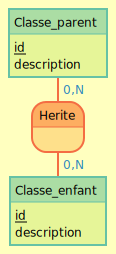
\includegraphics{mocodo/Classe_enfants/Classe_enfants.png}
\caption{Classe\_enfants.png}
\end{figure}

\begin{itemize}
\item
  Avec une entité-association réflexive :
  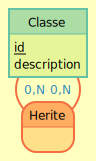
\includegraphics{mocodo/Classes/Classes.png}
\item
  Avec \href{https://mermaid-js.github.io/mermaid-live-editor/}{Mermaid}
  (je n'arrive pas à insérerer les attibuts pour l'entité) :
\end{itemize}

\href{https://mermaid-js.github.io/mermaid-live-editor/\#/edit/eyJjb2RlIjoiZXJEaWFncmFtXG4gICAgICAgIENsYXNzZSB9by0tb3sgQ2xhc3NlIDogSGVyaXRlXG4gICAgICAgIFxuXHRcdFx0XHRcdCIsIm1lcm1haWQiOnsidGhlbWUiOiJkZWZhdWx0In0sInVwZGF0ZUVkaXRvciI6ZmFsc2V9}{\includegraphics{https://mermaid.ink/img/eyJjb2RlIjoiZXJEaWFncmFtXG4gICAgICAgIENsYXNzZSB9by0tb3sgQ2xhc3NlIDogSGVyaXRlXG4gICAgICAgIFxuXHRcdFx0XHRcdCIsIm1lcm1haWQiOnsidGhlbWUiOiJkZWZhdWx0In0sInVwZGF0ZUVkaXRvciI6ZmFsc2V9}}

    \begin{itemize}
\tightlist
\item
  Diagramme de classes :
\end{itemize}

\href{https://mermaid-js.github.io/mermaid-live-editor/\#/edit/eyJjb2RlIjoiY2xhc3NEaWFncmFtXG5cdENob3NlIDx8LS0gQW5pbWFsXG5cdEFuaW1hbCA8fC0tIEh1bWFpblxuXHRIdW1haW4gPHwtLSBFbnNlaWduYW50XG5cdEFuaW1hbCA8fC0tIENoYXRcblx0U2NpZW5jZSA8fC0tIEVuc2VpZ25hbnRcblx0XG5cdFxuXHRcdFx0XHRcdCIsIm1lcm1haWQiOnsidGhlbWUiOiJkZWZhdWx0In0sInVwZGF0ZUVkaXRvciI6ZmFsc2V9}{\includegraphics{https://mermaid.ink/img/eyJjb2RlIjoiY2xhc3NEaWFncmFtXG5cdENob3NlIDx8LS0gQW5pbWFsXG5cdEFuaW1hbCA8fC0tIEh1bWFpblxuXHRIdW1haW4gPHwtLSBFbnNlaWduYW50XG5cdEFuaW1hbCA8fC0tIENoYXRcblx0U2NpZW5jZSA8fC0tIEVuc2VpZ25hbnRcblx0XG5cdFxuXHRcdFx0XHRcdCIsIm1lcm1haWQiOnsidGhlbWUiOiJkZWZhdWx0In0sInVwZGF0ZUVkaXRvciI6ZmFsc2V9}}

    \textbf{Exercice} : si on remplace
\texttt{PRIMARY\ KEY\ (enfant,\ parent)} par la contrainte
\texttt{PRIMARY\ KEY\ (enfant)} dans la définition de \texttt{Herite} :

\begin{itemize}
\tightlist
\item
  quelle restriction est imposée sur les hiérarchies de classes que
  cette base peut représenter ?
\end{itemize}

\begin{quote}
Voir ci-dessous, on ne peut pas insérer dans la table \texttt{Herite}
deux relations d'héritage avec le même identifiant \texttt{enfant} et
des identifiants \texttt{parent} distincts. Autrement dit, un enfant ne
peut avoir qu'un parent, une classe enfant ne peut hériter que d'une
seule classe mère.
\end{quote}

\begin{itemize}
\tightlist
\item
  quel est le changement correspondant dans le diagramme E/A ?
  \textgreater{} Changement de cardinalité sur l'une des pattes de
  l'association \texttt{Herite}, et séparation de l'entité
  \texttt{Classe} en deux entités \texttt{Classe\_parent} et
  \texttt{Classe\_enfant}. L'entité association estune relation
  fonctionnelle entre \texttt{Classe\_enfant} et
  \texttt{Classe\_parent}.
\end{itemize}

\begin{figure}
\centering
\includegraphics{mocodo/Classe_parents/Classe_parents.png}
\caption{Classe\_parents.png}
\end{figure}

\begin{itemize}
\tightlist
\item
  si on retraduit le diagramme E/A en schéma SQL, quel schéma
  obtiendra-t'on ?
\end{itemize}

\begin{quote}
Avec \href{http://mocodo.wingi.net/}{Mocodo}, on obtient un schéma avec
deux classes \texttt{Classe\_Enfant} et \texttt{Classe\_Parent} :
\end{quote}

\hypertarget{mld}{}
{Classe\_Enfant} ( {id}, {description}, {id.1} )

Le champ id constitue la clef primaire de la table. C'était déjà un
identifiant de l'entité Classe\_Enfant.

Le champ description était déjà un simple attribut de l'entité
Classe\_Enfant.

Le champ id.1 est une clef étrangère. Il a migré à partir de l'entité
Classe\_Parent par l'association de dépendance fonctionnelle Herite en
perdant son caractère identifiant.

{Classe\_Parent} ( {id}, {description} )

Le champ id constitue la clef primaire de la table. C'était déjà un
identifiant de l'entité Classe\_Parent.

Le champ description était déjà un simple attribut de l'entité
Classe\_Parent.

\begin{Shaded}
\begin{Highlighting}[]
\NormalTok{.}\KeywordTok{open} \OtherTok{"CLASSE\_ENFANTS"}\NormalTok{;}

\KeywordTok{CREATE} \KeywordTok{TABLE} \OtherTok{"CLASSE\_ENFANT"}\NormalTok{ (}
  \OtherTok{"id"} \DataTypeTok{VARCHAR}\NormalTok{(}\DecValTok{42}\NormalTok{),}
  \OtherTok{"description"} \DataTypeTok{VARCHAR}\NormalTok{(}\DecValTok{42}\NormalTok{),}
  \OtherTok{"id\_1"} \DataTypeTok{VARCHAR}\NormalTok{(}\DecValTok{42}\NormalTok{),}
  \KeywordTok{PRIMARY} \KeywordTok{KEY}\NormalTok{ (}\OtherTok{"id"}\NormalTok{),}
  \KeywordTok{FOREIGN} \KeywordTok{KEY}\NormalTok{ (}\OtherTok{"id\_1"}\NormalTok{) }\KeywordTok{REFERENCES} \OtherTok{"CLASSE\_PARENT"}\NormalTok{ (}\OtherTok{"id"}\NormalTok{)}
\NormalTok{);}

\KeywordTok{CREATE} \KeywordTok{TABLE} \OtherTok{"CLASSE\_PARENT"}\NormalTok{ (}
  \OtherTok{"id"} \DataTypeTok{VARCHAR}\NormalTok{(}\DecValTok{42}\NormalTok{),}
  \OtherTok{"description"} \DataTypeTok{VARCHAR}\NormalTok{(}\DecValTok{42}\NormalTok{),}
  \KeywordTok{PRIMARY} \KeywordTok{KEY}\NormalTok{ (}\OtherTok{"id"}\NormalTok{)}
\NormalTok{);}
\end{Highlighting}
\end{Shaded}

    \begin{Verbatim}[commandchars=\\\{\}]
{\color{incolor}In [{\color{incolor}49}]:} \PY{o}{\PYZpc{}}\PY{k}{sql} sqlite:///exo1\PYZhy{}q2.db
\end{Verbatim}


    \begin{Verbatim}[commandchars=\\\{\}]
{\color{incolor}In [{\color{incolor} }]:} \PY{o}{\PYZpc{}\PYZpc{}}\PY{k}{sql}
        
        PRAGMA foreign\PYZus{}keys=1;
\end{Verbatim}


    \begin{Verbatim}[commandchars=\\\{\}]
{\color{incolor}In [{\color{incolor}50}]:} \PY{o}{\PYZpc{}\PYZpc{}}\PY{k}{sql}
         
         CREATE TABLE Classe(
           id INTEGER PRIMARY KEY,
           description TEXT
         );
         
         CREATE TABLE Herite(
           enfant INT REFERENCES Classe(id),
           parent INT REFERENCES Classe(id),
           PRIMARY KEY (enfant)
         );
         
         INSERT INTO Classe VALUES(0, \PYZsq{}chose\PYZsq{});
         INSERT INTO Classe VALUES(1, \PYZsq{}animal\PYZsq{});
         INSERT INTO Classe VALUES(2, \PYZsq{}humain\PYZsq{});
         INSERT INTO Classe VALUES(3, \PYZsq{}enseignant\PYZsq{});
         INSERT INTO Classe VALUES(4, \PYZsq{}chat\PYZsq{});
         INSERT INTO Classe VALUES(5, \PYZsq{}science\PYZsq{});
         
         INSERT INTO Herite VALUES(1, 0);
         INSERT INTO Herite VALUES(2, 1);
         INSERT INTO Herite VALUES(3, 2);
         INSERT INTO Herite VALUES(4, 1);
         INSERT INTO Herite VALUES(3, 5);
\end{Verbatim}


    \begin{Verbatim}[commandchars=\\\{\}]
Done.
Done.
1 rows affected.
1 rows affected.
1 rows affected.
1 rows affected.
1 rows affected.
1 rows affected.
1 rows affected.
1 rows affected.
1 rows affected.
1 rows affected.

    \end{Verbatim}

    \begin{Verbatim}[commandchars=\\\{\}]

        ---------------------------------------------------------------------------

        IntegrityError                            Traceback (most recent call last)

        \textasciitilde{}/.local/lib/python3.6/site-packages/sqlalchemy/engine/base.py in \_execute\_context(self, dialect, constructor, statement, parameters, *args)
       1283                     self.dialect.do\_execute(
    -> 1284                         cursor, statement, parameters, context
       1285                     )


        \textasciitilde{}/.local/lib/python3.6/site-packages/sqlalchemy/engine/default.py in do\_execute(self, cursor, statement, parameters, context)
        589     def do\_execute(self, cursor, statement, parameters, context=None):
    --> 590         cursor.execute(statement, parameters)
        591 


        IntegrityError: UNIQUE constraint failed: Herite.enfant

        
    The above exception was the direct cause of the following exception:


        IntegrityError                            Traceback (most recent call last)

        <ipython-input-50-d034daf404cb> in <module>
    ----> 1 get\_ipython().run\_cell\_magic('sql', '', "\textbackslash{}nCREATE TABLE Classe(\textbackslash{}n  id INTEGER PRIMARY KEY,\textbackslash{}n  description TEXT\textbackslash{}n);\textbackslash{}n\textbackslash{}nCREATE TABLE Herite(\textbackslash{}n  enfant INT REFERENCES Classe(id),\textbackslash{}n  parent INT REFERENCES Classe(id),\textbackslash{}n  PRIMARY KEY (enfant)\textbackslash{}n);\textbackslash{}n\textbackslash{}nINSERT INTO Classe VALUES(0, 'chose');\textbackslash{}nINSERT INTO Classe VALUES(1, 'animal');\textbackslash{}nINSERT INTO Classe VALUES(2, 'humain');\textbackslash{}nINSERT INTO Classe VALUES(3, 'enseignant');\textbackslash{}nINSERT INTO Classe VALUES(4, 'chat');\textbackslash{}nINSERT INTO Classe VALUES(5, 'science');\textbackslash{}n\textbackslash{}nINSERT INTO Herite VALUES(1, 0);\textbackslash{}nINSERT INTO Herite VALUES(2, 1);\textbackslash{}nINSERT INTO Herite VALUES(3, 2);\textbackslash{}nINSERT INTO Herite VALUES(4, 1);\textbackslash{}nINSERT INTO Herite VALUES(3, 5);\textbackslash{}n")
    

        \textasciitilde{}/.local/lib/python3.6/site-packages/IPython/core/interactiveshell.py in run\_cell\_magic(self, magic\_name, line, cell)
       2360     def system\_raw(self, cmd):
       2361         """Call the given cmd in a subprocess using os.system on Windows or
    -> 2362         subprocess.call using the system shell on other platforms.
       2363 
       2364         Parameters


        <decorator-gen-157> in execute(self, line, cell, local\_ns)


        \textasciitilde{}/.local/lib/python3.6/site-packages/IPython/core/magic.py in <lambda>(f, *a, **k)
        185     """Decorator factory for methods in Magics subclasses.
        186     """
    --> 187 
        188     validate\_type(magic\_kind)
        189 


        <decorator-gen-156> in execute(self, line, cell, local\_ns)


        \textasciitilde{}/.local/lib/python3.6/site-packages/IPython/core/magic.py in <lambda>(f, *a, **k)
        185     """Decorator factory for methods in Magics subclasses.
        186     """
    --> 187 
        188     validate\_type(magic\_kind)
        189 


        \textasciitilde{}/.local/lib/python3.6/site-packages/sql/magic.py in execute(self, line, cell, local\_ns)
        215 
        216         try:
    --> 217             result = sql.run.run(conn, parsed["sql"], self, user\_ns)
        218 
        219             if (


        \textasciitilde{}/.local/lib/python3.6/site-packages/sql/run.py in run(conn, sql, config, user\_namespace)
        365             else:
        366                 txt = sqlalchemy.sql.text(statement)
    --> 367                 result = conn.session.execute(txt, user\_namespace)
        368             \_commit(conn=conn, config=config)
        369             if result and config.feedback:


        \textasciitilde{}/.local/lib/python3.6/site-packages/sqlalchemy/engine/base.py in execute(self, object\_, *multiparams, **params)
       1018             )
       1019         else:
    -> 1020             return meth(self, multiparams, params)
       1021 
       1022     def \_execute\_function(self, func, multiparams, params):


        \textasciitilde{}/.local/lib/python3.6/site-packages/sqlalchemy/sql/elements.py in \_execute\_on\_connection(self, connection, multiparams, params)
        296     def \_execute\_on\_connection(self, connection, multiparams, params):
        297         if self.supports\_execution:
    --> 298             return connection.\_execute\_clauseelement(self, multiparams, params)
        299         else:
        300             raise exc.ObjectNotExecutableError(self)


        \textasciitilde{}/.local/lib/python3.6/site-packages/sqlalchemy/engine/base.py in \_execute\_clauseelement(self, elem, multiparams, params)
       1137             distilled\_params,
       1138             compiled\_sql,
    -> 1139             distilled\_params,
       1140         )
       1141         if self.\_has\_events or self.engine.\_has\_events:


        \textasciitilde{}/.local/lib/python3.6/site-packages/sqlalchemy/engine/base.py in \_execute\_context(self, dialect, constructor, statement, parameters, *args)
       1322         except BaseException as e:
       1323             self.\_handle\_dbapi\_exception(
    -> 1324                 e, statement, parameters, cursor, context
       1325             )
       1326 


        \textasciitilde{}/.local/lib/python3.6/site-packages/sqlalchemy/engine/base.py in \_handle\_dbapi\_exception(self, e, statement, parameters, cursor, context)
       1516             elif should\_wrap:
       1517                 util.raise\_(
    -> 1518                     sqlalchemy\_exception, with\_traceback=exc\_info[2], from\_=e
       1519                 )
       1520             else:


        \textasciitilde{}/.local/lib/python3.6/site-packages/sqlalchemy/util/compat.py in raise\_(***failed resolving arguments***)
        176 
        177         try:
    --> 178             raise exception
        179         finally:
        180             \# credit to


        \textasciitilde{}/.local/lib/python3.6/site-packages/sqlalchemy/engine/base.py in \_execute\_context(self, dialect, constructor, statement, parameters, *args)
       1282                 if not evt\_handled:
       1283                     self.dialect.do\_execute(
    -> 1284                         cursor, statement, parameters, context
       1285                     )
       1286 


        \textasciitilde{}/.local/lib/python3.6/site-packages/sqlalchemy/engine/default.py in do\_execute(self, cursor, statement, parameters, context)
        588 
        589     def do\_execute(self, cursor, statement, parameters, context=None):
    --> 590         cursor.execute(statement, parameters)
        591 
        592     def do\_execute\_no\_params(self, cursor, statement, context=None):


        IntegrityError: (sqlite3.IntegrityError) UNIQUE constraint failed: Herite.enfant
    [SQL: INSERT INTO Herite VALUES(3, 5);]
    (Background on this error at: http://sqlalche.me/e/gkpj)

    \end{Verbatim}

    \textbf{Exercice} : mêmes questions que précédemment si on remplace
\texttt{PRIMARY\ KEY\ (enfant,\ parent)} par la contrainte
\texttt{PRIMARY\ KEY\ (parent)} .

\begin{itemize}
\tightlist
\item
  quelle restriction est imposée sur les hiérarchies de classes que
  cette base peut représenter ?
\end{itemize}

\begin{quote}
Voir ci-dessous, on ne peut pas insérer dans la table \texttt{Herite}
deux relations d'héritage avec le même identifiant \texttt{parent} et
des identifiants \texttt{enfant} distincts. Autrement dit, un parent ne
peut avoir qu'un enfant.
\end{quote}

\begin{verbatim}
IntegrityError: (sqlite3.IntegrityError) UNIQUE constraint failed: Herite.parent
[SQL: INSERT INTO Herite VALUES(4, 1);]
\end{verbatim}

\begin{itemize}
\tightlist
\item
  quel est le changement correspondant dans le diagramme E/A ?
  \textgreater{} Changement de cardinalité sur l'une des pattes de
  l'association \texttt{Herite}, et séparation de l'entité
  \texttt{Classe} en deux entités \texttt{Classe\_parent} et
  \texttt{Classe\_enfant}. L'entité association estune relation
  fonctionnelle entre \texttt{Classe\_parent} et
  \texttt{Classe\_enfant}.
\end{itemize}

\begin{figure}
\centering
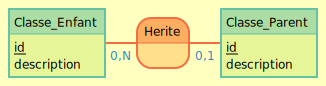
\includegraphics{mocodo/Classe_enfants2/Classe_enfants2.png}
\caption{Classe\_parents.png}
\end{figure}

\begin{itemize}
\tightlist
\item
  si on retraduit le diagramme E/A en schéma SQL, quel schéma
  obtiendra-t'on ?
\end{itemize}

\begin{quote}
Avec \href{http://mocodo.wingi.net/}{Mocodo}, on obtient un schéma deux
classes \texttt{Classe\_Enfant\textbackslash{}\ et}Classe\_Parent` :
\end{quote}

\hypertarget{mld}{}
{Classe\_Enfant} ( {id}, {description}, {id.1} )

Le champ id constitue la clef primaire de la table. C'était déjà un
identifiant de l'entité Classe\_Enfant.

Le champ description était déjà un simple attribut de l'entité
Classe\_Enfant.

Le champ id.1 est une clef étrangère. Il a migré à partir de l'entité
Classe\_Parent par l'association de dépendance fonctionnelle Herite en
perdant son caractère identifiant.

{Classe\_Parent} ( {id}, {description} )

Le champ id constitue la clef primaire de la table. C'était déjà un
identifiant de l'entité Classe\_Parent.

Le champ description était déjà un simple attribut de l'entité
Classe\_Parent.

\begin{Shaded}
\begin{Highlighting}[]
\NormalTok{.}\KeywordTok{open} \OtherTok{"CLASSE\_ENFANTS"}\NormalTok{;}

\KeywordTok{CREATE} \KeywordTok{TABLE} \OtherTok{"CLASSE\_ENFANT"}\NormalTok{ (}
  \OtherTok{"id"} \DataTypeTok{VARCHAR}\NormalTok{(}\DecValTok{42}\NormalTok{),}
  \OtherTok{"description"} \DataTypeTok{VARCHAR}\NormalTok{(}\DecValTok{42}\NormalTok{),}
  \OtherTok{"id\_1"} \DataTypeTok{VARCHAR}\NormalTok{(}\DecValTok{42}\NormalTok{),}
  \KeywordTok{PRIMARY} \KeywordTok{KEY}\NormalTok{ (}\OtherTok{"id"}\NormalTok{),}
  \KeywordTok{FOREIGN} \KeywordTok{KEY}\NormalTok{ (}\OtherTok{"id\_1"}\NormalTok{) }\KeywordTok{REFERENCES} \OtherTok{"CLASSE\_PARENT"}\NormalTok{ (}\OtherTok{"id"}\NormalTok{)}
\NormalTok{);}

\KeywordTok{CREATE} \KeywordTok{TABLE} \OtherTok{"CLASSE\_PARENT"}\NormalTok{ (}
  \OtherTok{"id"} \DataTypeTok{VARCHAR}\NormalTok{(}\DecValTok{42}\NormalTok{),}
  \OtherTok{"description"} \DataTypeTok{VARCHAR}\NormalTok{(}\DecValTok{42}\NormalTok{),}
  \KeywordTok{PRIMARY} \KeywordTok{KEY}\NormalTok{ (}\OtherTok{"id"}\NormalTok{)}
\NormalTok{);}
\end{Highlighting}
\end{Shaded}

    \begin{Verbatim}[commandchars=\\\{\}]
{\color{incolor}In [{\color{incolor}51}]:} \PY{o}{\PYZpc{}}\PY{k}{sql} sqlite:///exo1\PYZhy{}q3.db
\end{Verbatim}


    \begin{Verbatim}[commandchars=\\\{\}]
{\color{incolor}In [{\color{incolor}90}]:} \PY{o}{\PYZpc{}\PYZpc{}}\PY{k}{sql}
         
         PRAGMA foreign\PYZus{}keys=1;
\end{Verbatim}


    \begin{Verbatim}[commandchars=\\\{\}]
Done.

    \end{Verbatim}

\begin{Verbatim}[commandchars=\\\{\}]
{\color{outcolor}Out[{\color{outcolor}90}]:} []
\end{Verbatim}
            
    \begin{Verbatim}[commandchars=\\\{\}]
{\color{incolor}In [{\color{incolor}52}]:} \PY{o}{\PYZpc{}\PYZpc{}}\PY{k}{sql}
         
         CREATE TABLE Classe(
           id INTEGER PRIMARY KEY,
           description TEXT
         );
         
         CREATE TABLE Herite(
           enfant INT REFERENCES Classe(id),
           parent INT REFERENCES Classe(id),
           PRIMARY KEY (parent)
         );
         
         INSERT INTO Classe VALUES(0, \PYZsq{}chose\PYZsq{});
         INSERT INTO Classe VALUES(1, \PYZsq{}animal\PYZsq{});
         INSERT INTO Classe VALUES(2, \PYZsq{}humain\PYZsq{});
         INSERT INTO Classe VALUES(3, \PYZsq{}enseignant\PYZsq{});
         INSERT INTO Classe VALUES(4, \PYZsq{}chat\PYZsq{});
         INSERT INTO Classe VALUES(5, \PYZsq{}science\PYZsq{});
         
         INSERT INTO Herite VALUES(1, 0);
         INSERT INTO Herite VALUES(2, 1);
         INSERT INTO Herite VALUES(3, 2);
         INSERT INTO Herite VALUES(4, 1);
         INSERT INTO Herite VALUES(3, 5);
\end{Verbatim}


    \begin{Verbatim}[commandchars=\\\{\}]
Done.
Done.
1 rows affected.
1 rows affected.
1 rows affected.
1 rows affected.
1 rows affected.
1 rows affected.
1 rows affected.
1 rows affected.
1 rows affected.

    \end{Verbatim}

    \begin{Verbatim}[commandchars=\\\{\}]

        ---------------------------------------------------------------------------

        IntegrityError                            Traceback (most recent call last)

        \textasciitilde{}/.local/lib/python3.6/site-packages/sqlalchemy/engine/base.py in \_execute\_context(self, dialect, constructor, statement, parameters, *args)
       1283                     self.dialect.do\_execute(
    -> 1284                         cursor, statement, parameters, context
       1285                     )


        \textasciitilde{}/.local/lib/python3.6/site-packages/sqlalchemy/engine/default.py in do\_execute(self, cursor, statement, parameters, context)
        589     def do\_execute(self, cursor, statement, parameters, context=None):
    --> 590         cursor.execute(statement, parameters)
        591 


        IntegrityError: UNIQUE constraint failed: Herite.parent

        
    The above exception was the direct cause of the following exception:


        IntegrityError                            Traceback (most recent call last)

        <ipython-input-52-e73c42513e64> in <module>
    ----> 1 get\_ipython().run\_cell\_magic('sql', '', "\textbackslash{}nCREATE TABLE Classe(\textbackslash{}n  id INTEGER PRIMARY KEY,\textbackslash{}n  description TEXT\textbackslash{}n);\textbackslash{}n\textbackslash{}nCREATE TABLE Herite(\textbackslash{}n  enfant INT REFERENCES Classe(id),\textbackslash{}n  parent INT REFERENCES Classe(id),\textbackslash{}n  PRIMARY KEY (parent)\textbackslash{}n);\textbackslash{}n\textbackslash{}nINSERT INTO Classe VALUES(0, 'chose');\textbackslash{}nINSERT INTO Classe VALUES(1, 'animal');\textbackslash{}nINSERT INTO Classe VALUES(2, 'humain');\textbackslash{}nINSERT INTO Classe VALUES(3, 'enseignant');\textbackslash{}nINSERT INTO Classe VALUES(4, 'chat');\textbackslash{}nINSERT INTO Classe VALUES(5, 'science');\textbackslash{}n\textbackslash{}nINSERT INTO Herite VALUES(1, 0);\textbackslash{}nINSERT INTO Herite VALUES(2, 1);\textbackslash{}nINSERT INTO Herite VALUES(3, 2);\textbackslash{}nINSERT INTO Herite VALUES(4, 1);\textbackslash{}nINSERT INTO Herite VALUES(3, 5);\textbackslash{}n")
    

        \textasciitilde{}/.local/lib/python3.6/site-packages/IPython/core/interactiveshell.py in run\_cell\_magic(self, magic\_name, line, cell)
       2360     def system\_raw(self, cmd):
       2361         """Call the given cmd in a subprocess using os.system on Windows or
    -> 2362         subprocess.call using the system shell on other platforms.
       2363 
       2364         Parameters


        <decorator-gen-157> in execute(self, line, cell, local\_ns)


        \textasciitilde{}/.local/lib/python3.6/site-packages/IPython/core/magic.py in <lambda>(f, *a, **k)
        185     """Decorator factory for methods in Magics subclasses.
        186     """
    --> 187 
        188     validate\_type(magic\_kind)
        189 


        <decorator-gen-156> in execute(self, line, cell, local\_ns)


        \textasciitilde{}/.local/lib/python3.6/site-packages/IPython/core/magic.py in <lambda>(f, *a, **k)
        185     """Decorator factory for methods in Magics subclasses.
        186     """
    --> 187 
        188     validate\_type(magic\_kind)
        189 


        \textasciitilde{}/.local/lib/python3.6/site-packages/sql/magic.py in execute(self, line, cell, local\_ns)
        215 
        216         try:
    --> 217             result = sql.run.run(conn, parsed["sql"], self, user\_ns)
        218 
        219             if (


        \textasciitilde{}/.local/lib/python3.6/site-packages/sql/run.py in run(conn, sql, config, user\_namespace)
        365             else:
        366                 txt = sqlalchemy.sql.text(statement)
    --> 367                 result = conn.session.execute(txt, user\_namespace)
        368             \_commit(conn=conn, config=config)
        369             if result and config.feedback:


        \textasciitilde{}/.local/lib/python3.6/site-packages/sqlalchemy/engine/base.py in execute(self, object\_, *multiparams, **params)
       1018             )
       1019         else:
    -> 1020             return meth(self, multiparams, params)
       1021 
       1022     def \_execute\_function(self, func, multiparams, params):


        \textasciitilde{}/.local/lib/python3.6/site-packages/sqlalchemy/sql/elements.py in \_execute\_on\_connection(self, connection, multiparams, params)
        296     def \_execute\_on\_connection(self, connection, multiparams, params):
        297         if self.supports\_execution:
    --> 298             return connection.\_execute\_clauseelement(self, multiparams, params)
        299         else:
        300             raise exc.ObjectNotExecutableError(self)


        \textasciitilde{}/.local/lib/python3.6/site-packages/sqlalchemy/engine/base.py in \_execute\_clauseelement(self, elem, multiparams, params)
       1137             distilled\_params,
       1138             compiled\_sql,
    -> 1139             distilled\_params,
       1140         )
       1141         if self.\_has\_events or self.engine.\_has\_events:


        \textasciitilde{}/.local/lib/python3.6/site-packages/sqlalchemy/engine/base.py in \_execute\_context(self, dialect, constructor, statement, parameters, *args)
       1322         except BaseException as e:
       1323             self.\_handle\_dbapi\_exception(
    -> 1324                 e, statement, parameters, cursor, context
       1325             )
       1326 


        \textasciitilde{}/.local/lib/python3.6/site-packages/sqlalchemy/engine/base.py in \_handle\_dbapi\_exception(self, e, statement, parameters, cursor, context)
       1516             elif should\_wrap:
       1517                 util.raise\_(
    -> 1518                     sqlalchemy\_exception, with\_traceback=exc\_info[2], from\_=e
       1519                 )
       1520             else:


        \textasciitilde{}/.local/lib/python3.6/site-packages/sqlalchemy/util/compat.py in raise\_(***failed resolving arguments***)
        176 
        177         try:
    --> 178             raise exception
        179         finally:
        180             \# credit to


        \textasciitilde{}/.local/lib/python3.6/site-packages/sqlalchemy/engine/base.py in \_execute\_context(self, dialect, constructor, statement, parameters, *args)
       1282                 if not evt\_handled:
       1283                     self.dialect.do\_execute(
    -> 1284                         cursor, statement, parameters, context
       1285                     )
       1286 


        \textasciitilde{}/.local/lib/python3.6/site-packages/sqlalchemy/engine/default.py in do\_execute(self, cursor, statement, parameters, context)
        588 
        589     def do\_execute(self, cursor, statement, parameters, context=None):
    --> 590         cursor.execute(statement, parameters)
        591 
        592     def do\_execute\_no\_params(self, cursor, statement, context=None):


        IntegrityError: (sqlite3.IntegrityError) UNIQUE constraint failed: Herite.parent
    [SQL: INSERT INTO Herite VALUES(4, 1);]
    (Background on this error at: http://sqlalche.me/e/gkpj)

    \end{Verbatim}

    \textbf{Exercice} : mêmes questions que précédemment si on enlève
simplement la contrainte \texttt{PRIMARY\ KEY\ (enfant,\ parent)}.

    \begin{Verbatim}[commandchars=\\\{\}]
{\color{incolor}In [{\color{incolor}106}]:} \PY{o}{\PYZpc{}}\PY{k}{sql} sqlite:///exo1\PYZhy{}q10.db
\end{Verbatim}


    \begin{Verbatim}[commandchars=\\\{\}]
{\color{incolor}In [{\color{incolor}107}]:} \PY{o}{\PYZpc{}\PYZpc{}}\PY{k}{sql}
          
          PRAGMA foreign\PYZus{}keys=1;
\end{Verbatim}


    \begin{Verbatim}[commandchars=\\\{\}]
Done.

    \end{Verbatim}

\begin{Verbatim}[commandchars=\\\{\}]
{\color{outcolor}Out[{\color{outcolor}107}]:} []
\end{Verbatim}
            
    \begin{Verbatim}[commandchars=\\\{\}]
{\color{incolor}In [{\color{incolor}108}]:} \PY{o}{\PYZpc{}\PYZpc{}}\PY{k}{sql}
          
          CREATE TABLE Classe(
            id INTEGER PRIMARY KEY,
            description TEXT
          );
          
          CREATE TABLE Herite(
            enfant INT REFERENCES Classe(id),
            parent INT REFERENCES Classe(id)
              )
          ;
          
          INSERT INTO Classe VALUES(0, \PYZsq{}chose\PYZsq{});
          INSERT INTO Classe VALUES(1, \PYZsq{}animal\PYZsq{});
          INSERT INTO Classe VALUES(2, \PYZsq{}humain\PYZsq{});
          INSERT INTO Classe VALUES(3, \PYZsq{}enseignant\PYZsq{});
          INSERT INTO Classe VALUES(4, \PYZsq{}chat\PYZsq{});
          INSERT INTO Classe VALUES(5, \PYZsq{}science\PYZsq{});
          
          INSERT INTO Herite VALUES(1, 0);
          INSERT INTO Herite VALUES(2, 1);
          INSERT INTO Herite VALUES(3, 2);
          INSERT INTO Herite VALUES(4, 1);
          INSERT INTO Herite VALUES(3, 5);
\end{Verbatim}


    \begin{Verbatim}[commandchars=\\\{\}]
Done.
Done.
1 rows affected.
1 rows affected.
1 rows affected.
1 rows affected.
1 rows affected.
1 rows affected.
1 rows affected.
1 rows affected.
1 rows affected.
1 rows affected.
1 rows affected.

    \end{Verbatim}

\begin{Verbatim}[commandchars=\\\{\}]
{\color{outcolor}Out[{\color{outcolor}108}]:} []
\end{Verbatim}
            
    On a toujours une contrainte d'intégrité avec la clef \texttt{id} dans
la table \texttt{Classe}, on ne peut pas insérer un tuple avec un
\texttt{id} déjà attibué

    \begin{Verbatim}[commandchars=\\\{\}]
{\color{incolor}In [{\color{incolor}109}]:} \PY{o}{\PYZpc{}\PYZpc{}}\PY{k}{sql}
          
          INSERT INTO Classe VALUES(0, \PYZsq{}patate\PYZsq{});
          
          \PYZhy{}\PYZhy{} IntegrityError: (sqlite3.IntegrityError) UNIQUE constraint failed: Classe.id
          [SQL: INSERT INTO Classe VALUES(0, \PYZsq{}patate\PYZsq{});]
\end{Verbatim}


    \begin{Verbatim}[commandchars=\\\{\}]

        ---------------------------------------------------------------------------

        IntegrityError                            Traceback (most recent call last)

        \textasciitilde{}/.local/lib/python3.6/site-packages/sqlalchemy/engine/base.py in \_execute\_context(self, dialect, constructor, statement, parameters, *args)
       1283                     self.dialect.do\_execute(
    -> 1284                         cursor, statement, parameters, context
       1285                     )


        \textasciitilde{}/.local/lib/python3.6/site-packages/sqlalchemy/engine/default.py in do\_execute(self, cursor, statement, parameters, context)
        589     def do\_execute(self, cursor, statement, parameters, context=None):
    --> 590         cursor.execute(statement, parameters)
        591 


        IntegrityError: UNIQUE constraint failed: Classe.id

        
    The above exception was the direct cause of the following exception:


        IntegrityError                            Traceback (most recent call last)

        <ipython-input-109-13f5cdc438b7> in <module>
    ----> 1 get\_ipython().run\_cell\_magic('sql', '', "\textbackslash{}nINSERT INTO Classe VALUES(0, 'patate');\textbackslash{}n\textbackslash{}n-- IntegrityError: (sqlite3.IntegrityError) UNIQUE constraint failed: Classe.id\textbackslash{}n[SQL: INSERT INTO Classe VALUES(0, 'patate');]\textbackslash{}n")
    

        \textasciitilde{}/.local/lib/python3.6/site-packages/IPython/core/interactiveshell.py in run\_cell\_magic(self, magic\_name, line, cell)
       2360     def system\_raw(self, cmd):
       2361         """Call the given cmd in a subprocess using os.system on Windows or
    -> 2362         subprocess.call using the system shell on other platforms.
       2363 
       2364         Parameters


        <decorator-gen-157> in execute(self, line, cell, local\_ns)


        \textasciitilde{}/.local/lib/python3.6/site-packages/IPython/core/magic.py in <lambda>(f, *a, **k)
        185     """Decorator factory for methods in Magics subclasses.
        186     """
    --> 187 
        188     validate\_type(magic\_kind)
        189 


        <decorator-gen-156> in execute(self, line, cell, local\_ns)


        \textasciitilde{}/.local/lib/python3.6/site-packages/IPython/core/magic.py in <lambda>(f, *a, **k)
        185     """Decorator factory for methods in Magics subclasses.
        186     """
    --> 187 
        188     validate\_type(magic\_kind)
        189 


        \textasciitilde{}/.local/lib/python3.6/site-packages/sql/magic.py in execute(self, line, cell, local\_ns)
        215 
        216         try:
    --> 217             result = sql.run.run(conn, parsed["sql"], self, user\_ns)
        218 
        219             if (


        \textasciitilde{}/.local/lib/python3.6/site-packages/sql/run.py in run(conn, sql, config, user\_namespace)
        365             else:
        366                 txt = sqlalchemy.sql.text(statement)
    --> 367                 result = conn.session.execute(txt, user\_namespace)
        368             \_commit(conn=conn, config=config)
        369             if result and config.feedback:


        \textasciitilde{}/.local/lib/python3.6/site-packages/sqlalchemy/engine/base.py in execute(self, object\_, *multiparams, **params)
       1018             )
       1019         else:
    -> 1020             return meth(self, multiparams, params)
       1021 
       1022     def \_execute\_function(self, func, multiparams, params):


        \textasciitilde{}/.local/lib/python3.6/site-packages/sqlalchemy/sql/elements.py in \_execute\_on\_connection(self, connection, multiparams, params)
        296     def \_execute\_on\_connection(self, connection, multiparams, params):
        297         if self.supports\_execution:
    --> 298             return connection.\_execute\_clauseelement(self, multiparams, params)
        299         else:
        300             raise exc.ObjectNotExecutableError(self)


        \textasciitilde{}/.local/lib/python3.6/site-packages/sqlalchemy/engine/base.py in \_execute\_clauseelement(self, elem, multiparams, params)
       1137             distilled\_params,
       1138             compiled\_sql,
    -> 1139             distilled\_params,
       1140         )
       1141         if self.\_has\_events or self.engine.\_has\_events:


        \textasciitilde{}/.local/lib/python3.6/site-packages/sqlalchemy/engine/base.py in \_execute\_context(self, dialect, constructor, statement, parameters, *args)
       1322         except BaseException as e:
       1323             self.\_handle\_dbapi\_exception(
    -> 1324                 e, statement, parameters, cursor, context
       1325             )
       1326 


        \textasciitilde{}/.local/lib/python3.6/site-packages/sqlalchemy/engine/base.py in \_handle\_dbapi\_exception(self, e, statement, parameters, cursor, context)
       1516             elif should\_wrap:
       1517                 util.raise\_(
    -> 1518                     sqlalchemy\_exception, with\_traceback=exc\_info[2], from\_=e
       1519                 )
       1520             else:


        \textasciitilde{}/.local/lib/python3.6/site-packages/sqlalchemy/util/compat.py in raise\_(***failed resolving arguments***)
        176 
        177         try:
    --> 178             raise exception
        179         finally:
        180             \# credit to


        \textasciitilde{}/.local/lib/python3.6/site-packages/sqlalchemy/engine/base.py in \_execute\_context(self, dialect, constructor, statement, parameters, *args)
       1282                 if not evt\_handled:
       1283                     self.dialect.do\_execute(
    -> 1284                         cursor, statement, parameters, context
       1285                     )
       1286 


        \textasciitilde{}/.local/lib/python3.6/site-packages/sqlalchemy/engine/default.py in do\_execute(self, cursor, statement, parameters, context)
        588 
        589     def do\_execute(self, cursor, statement, parameters, context=None):
    --> 590         cursor.execute(statement, parameters)
        591 
        592     def do\_execute\_no\_params(self, cursor, statement, context=None):


        IntegrityError: (sqlite3.IntegrityError) UNIQUE constraint failed: Classe.id
    [SQL: INSERT INTO Classe VALUES(0, 'patate');]
    (Background on this error at: http://sqlalche.me/e/gkpj)

    \end{Verbatim}

    En revanche, on n'a plus de contrainte d'intégrité sur l'unicité dans la
table \texttt{Herite} (qui n'a plus de clef prmimaire).

    \begin{Verbatim}[commandchars=\\\{\}]
{\color{incolor}In [{\color{incolor}112}]:} \PY{o}{\PYZpc{}\PYZpc{}}\PY{k}{sql}
          
          INSERT INTO Herite VALUES(1, 0);
\end{Verbatim}


    \begin{Verbatim}[commandchars=\\\{\}]
1 rows affected.

    \end{Verbatim}

\begin{Verbatim}[commandchars=\\\{\}]
{\color{outcolor}Out[{\color{outcolor}112}]:} []
\end{Verbatim}
            
    On a toujours la contrainte d'intégrité référentielle entre les colonnes
\texttt{enfant} et \texttt{parent} de la table \texttt{Herite} et la
colonne \texttt{id} de la table \texttt{Classe} (contrainte de clef
étangère).

    \begin{Verbatim}[commandchars=\\\{\}]
{\color{incolor}In [{\color{incolor}110}]:} \PY{o}{\PYZpc{}\PYZpc{}}\PY{k}{sql}
          
          INSERT INTO Herite VALUES(1, 7);
          
          \PYZhy{}\PYZhy{}IntegrityError: (sqlite3.IntegrityError) FOREIGN KEY constraint failed
          [SQL: INSERT INTO Herite VALUES(1, 7);]
\end{Verbatim}


    \begin{Verbatim}[commandchars=\\\{\}]

        ---------------------------------------------------------------------------

        IntegrityError                            Traceback (most recent call last)

        \textasciitilde{}/.local/lib/python3.6/site-packages/sqlalchemy/engine/base.py in \_execute\_context(self, dialect, constructor, statement, parameters, *args)
       1283                     self.dialect.do\_execute(
    -> 1284                         cursor, statement, parameters, context
       1285                     )


        \textasciitilde{}/.local/lib/python3.6/site-packages/sqlalchemy/engine/default.py in do\_execute(self, cursor, statement, parameters, context)
        589     def do\_execute(self, cursor, statement, parameters, context=None):
    --> 590         cursor.execute(statement, parameters)
        591 


        IntegrityError: FOREIGN KEY constraint failed

        
    The above exception was the direct cause of the following exception:


        IntegrityError                            Traceback (most recent call last)

        <ipython-input-110-b5eb68a35a96> in <module>
    ----> 1 get\_ipython().run\_cell\_magic('sql', '', '\textbackslash{}nINSERT INTO Herite VALUES(1, 7);\textbackslash{}n')
    

        \textasciitilde{}/.local/lib/python3.6/site-packages/IPython/core/interactiveshell.py in run\_cell\_magic(self, magic\_name, line, cell)
       2360     def system\_raw(self, cmd):
       2361         """Call the given cmd in a subprocess using os.system on Windows or
    -> 2362         subprocess.call using the system shell on other platforms.
       2363 
       2364         Parameters


        <decorator-gen-157> in execute(self, line, cell, local\_ns)


        \textasciitilde{}/.local/lib/python3.6/site-packages/IPython/core/magic.py in <lambda>(f, *a, **k)
        185     """Decorator factory for methods in Magics subclasses.
        186     """
    --> 187 
        188     validate\_type(magic\_kind)
        189 


        <decorator-gen-156> in execute(self, line, cell, local\_ns)


        \textasciitilde{}/.local/lib/python3.6/site-packages/IPython/core/magic.py in <lambda>(f, *a, **k)
        185     """Decorator factory for methods in Magics subclasses.
        186     """
    --> 187 
        188     validate\_type(magic\_kind)
        189 


        \textasciitilde{}/.local/lib/python3.6/site-packages/sql/magic.py in execute(self, line, cell, local\_ns)
        215 
        216         try:
    --> 217             result = sql.run.run(conn, parsed["sql"], self, user\_ns)
        218 
        219             if (


        \textasciitilde{}/.local/lib/python3.6/site-packages/sql/run.py in run(conn, sql, config, user\_namespace)
        365             else:
        366                 txt = sqlalchemy.sql.text(statement)
    --> 367                 result = conn.session.execute(txt, user\_namespace)
        368             \_commit(conn=conn, config=config)
        369             if result and config.feedback:


        \textasciitilde{}/.local/lib/python3.6/site-packages/sqlalchemy/engine/base.py in execute(self, object\_, *multiparams, **params)
       1018             )
       1019         else:
    -> 1020             return meth(self, multiparams, params)
       1021 
       1022     def \_execute\_function(self, func, multiparams, params):


        \textasciitilde{}/.local/lib/python3.6/site-packages/sqlalchemy/sql/elements.py in \_execute\_on\_connection(self, connection, multiparams, params)
        296     def \_execute\_on\_connection(self, connection, multiparams, params):
        297         if self.supports\_execution:
    --> 298             return connection.\_execute\_clauseelement(self, multiparams, params)
        299         else:
        300             raise exc.ObjectNotExecutableError(self)


        \textasciitilde{}/.local/lib/python3.6/site-packages/sqlalchemy/engine/base.py in \_execute\_clauseelement(self, elem, multiparams, params)
       1137             distilled\_params,
       1138             compiled\_sql,
    -> 1139             distilled\_params,
       1140         )
       1141         if self.\_has\_events or self.engine.\_has\_events:


        \textasciitilde{}/.local/lib/python3.6/site-packages/sqlalchemy/engine/base.py in \_execute\_context(self, dialect, constructor, statement, parameters, *args)
       1322         except BaseException as e:
       1323             self.\_handle\_dbapi\_exception(
    -> 1324                 e, statement, parameters, cursor, context
       1325             )
       1326 


        \textasciitilde{}/.local/lib/python3.6/site-packages/sqlalchemy/engine/base.py in \_handle\_dbapi\_exception(self, e, statement, parameters, cursor, context)
       1516             elif should\_wrap:
       1517                 util.raise\_(
    -> 1518                     sqlalchemy\_exception, with\_traceback=exc\_info[2], from\_=e
       1519                 )
       1520             else:


        \textasciitilde{}/.local/lib/python3.6/site-packages/sqlalchemy/util/compat.py in raise\_(***failed resolving arguments***)
        176 
        177         try:
    --> 178             raise exception
        179         finally:
        180             \# credit to


        \textasciitilde{}/.local/lib/python3.6/site-packages/sqlalchemy/engine/base.py in \_execute\_context(self, dialect, constructor, statement, parameters, *args)
       1282                 if not evt\_handled:
       1283                     self.dialect.do\_execute(
    -> 1284                         cursor, statement, parameters, context
       1285                     )
       1286 


        \textasciitilde{}/.local/lib/python3.6/site-packages/sqlalchemy/engine/default.py in do\_execute(self, cursor, statement, parameters, context)
        588 
        589     def do\_execute(self, cursor, statement, parameters, context=None):
    --> 590         cursor.execute(statement, parameters)
        591 
        592     def do\_execute\_no\_params(self, cursor, statement, context=None):


        IntegrityError: (sqlite3.IntegrityError) FOREIGN KEY constraint failed
    [SQL: INSERT INTO Herite VALUES(1, 7);]
    (Background on this error at: http://sqlalche.me/e/gkpj)

    \end{Verbatim}

    \begin{Verbatim}[commandchars=\\\{\}]
{\color{incolor}In [{\color{incolor}96}]:} \PY{o}{\PYZpc{}\PYZpc{}}\PY{k}{sql}
         
         INSERT INTO Herite VALUES(1, 7);
\end{Verbatim}


    \begin{Verbatim}[commandchars=\\\{\}]
1 rows affected.

    \end{Verbatim}

\begin{Verbatim}[commandchars=\\\{\}]
{\color{outcolor}Out[{\color{outcolor}96}]:} []
\end{Verbatim}
            
    \begin{Verbatim}[commandchars=\\\{\}]
{\color{incolor}In [{\color{incolor}113}]:} \PY{o}{\PYZpc{}\PYZpc{}}\PY{k}{sql} 
          
          SELECT * FROM Herite;
\end{Verbatim}


    \begin{Verbatim}[commandchars=\\\{\}]
Done.

    \end{Verbatim}

\begin{Verbatim}[commandchars=\\\{\}]
{\color{outcolor}Out[{\color{outcolor}113}]:} [(1, 0), (2, 1), (3, 2), (4, 1), (3, 5), (1, 0)]
\end{Verbatim}
            
    \begin{Verbatim}[commandchars=\\\{\}]
{\color{incolor}In [{\color{incolor}114}]:} \PY{o}{\PYZpc{}\PYZpc{}}\PY{k}{sql} 
          
          SELECT * FROM Classe;
\end{Verbatim}


    \begin{Verbatim}[commandchars=\\\{\}]
Done.

    \end{Verbatim}

\begin{Verbatim}[commandchars=\\\{\}]
{\color{outcolor}Out[{\color{outcolor}114}]:} [(0, 'chose'),
           (1, 'animal'),
           (2, 'humain'),
           (3, 'enseignant'),
           (4, 'chat'),
           (5, 'science')]
\end{Verbatim}
            
    \begin{itemize}
\tightlist
\item
  Diagramme entité relation dans ce cas :
\end{itemize}

\begin{figure}
\centering
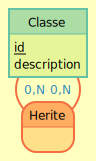
\includegraphics{mocodo/Classes/Classes.png}
\caption{Classe\_parents2.png}
\end{figure}

\begin{itemize}
\tightlist
\item
  Schéma SQL :
\end{itemize}

\hypertarget{mld}{}
{Classe} ( {id}, {description} )

Le champ id constitue la clef primaire de la table. C'était déjà un
identifiant de l'entité Classe.

Le champ description était déjà un simple attribut de l'entité Classe.

{Herite} ( {id}, {id.1} )

Les champs id et id.1 constituent la clef primaire de la table. Ce sont
des clefs étrangères qui ont migré directement à partir de l'entité
Classe.

\begin{Shaded}
\begin{Highlighting}[]
\NormalTok{.}\KeywordTok{open} \OtherTok{"CLASSES"}\NormalTok{;}

\KeywordTok{CREATE} \KeywordTok{TABLE} \OtherTok{"CLASSE"}\NormalTok{ (}
  \OtherTok{"id"} \DataTypeTok{VARCHAR}\NormalTok{(}\DecValTok{42}\NormalTok{),}
  \OtherTok{"description"} \DataTypeTok{VARCHAR}\NormalTok{(}\DecValTok{42}\NormalTok{),}
  \KeywordTok{PRIMARY} \KeywordTok{KEY}\NormalTok{ (}\OtherTok{"id"}\NormalTok{)}
\NormalTok{);}

\KeywordTok{CREATE} \KeywordTok{TABLE} \OtherTok{"HERITE"}\NormalTok{ (}
  \OtherTok{"id"} \DataTypeTok{VARCHAR}\NormalTok{(}\DecValTok{42}\NormalTok{),}
  \OtherTok{"id\_1"} \DataTypeTok{VARCHAR}\NormalTok{(}\DecValTok{42}\NormalTok{),}
  \KeywordTok{PRIMARY} \KeywordTok{KEY}\NormalTok{ (}\OtherTok{"id"}\NormalTok{, }\OtherTok{"id\_1"}\NormalTok{),}
  \KeywordTok{FOREIGN} \KeywordTok{KEY}\NormalTok{ (}\OtherTok{"id"}\NormalTok{) }\KeywordTok{REFERENCES} \OtherTok{"CLASSE"}\NormalTok{ (}\OtherTok{"id"}\NormalTok{),}
  \KeywordTok{FOREIGN} \KeywordTok{KEY}\NormalTok{ (}\OtherTok{"id\_1"}\NormalTok{) }\KeywordTok{REFERENCES} \OtherTok{"CLASSE"}\NormalTok{ (}\OtherTok{"id"}\NormalTok{)}
\NormalTok{);}
\end{Highlighting}
\end{Shaded}

    \hypertarget{exercice-2-reprise-de-la-base-stanford}{%
\subsection{\texorpdfstring{Exercice 2 : reprise de la base
\emph{Stanford}}{Exercice 2 : reprise de la base Stanford}}\label{exercice-2-reprise-de-la-base-stanford}}

On reprend la base \emph{Stanford} d'exemple de la première partie. Le
script de création de table est le suivant.

\begin{Shaded}
\begin{Highlighting}[]
\KeywordTok{create} \KeywordTok{table}\NormalTok{ College(}
\NormalTok{    cName }\DataTypeTok{varchar}\NormalTok{(}\DecValTok{255}\NormalTok{),}
\NormalTok{    state }\DataTypeTok{varchar}\NormalTok{(}\DecValTok{255}\NormalTok{),}
\NormalTok{    enrollment }\DataTypeTok{int}\NormalTok{);}
    
\KeywordTok{create} \KeywordTok{table}\NormalTok{ Student(}
\NormalTok{    sID }\DataTypeTok{int}\NormalTok{,}
\NormalTok{    sName }\DataTypeTok{varchar}\NormalTok{(}\DecValTok{255}\NormalTok{),}
\NormalTok{    GPA }\DataTypeTok{real}\NormalTok{, }\CommentTok{{-}{-} Grade Point Average, out of 4}
\NormalTok{    sizeHS }\DataTypeTok{int}\NormalTok{);}

\KeywordTok{create} \KeywordTok{table}\NormalTok{ Apply(}
\NormalTok{  sID }\DataTypeTok{int}\NormalTok{,}
\NormalTok{  cName }\DataTypeTok{varchar}\NormalTok{(}\DecValTok{255}\NormalTok{),}
\NormalTok{  major }\DataTypeTok{varchar}\NormalTok{(}\DecValTok{255}\NormalTok{),}
\NormalTok{  decision }\DataTypeTok{char}\NormalTok{(}\DecValTok{1}\NormalTok{));}
\end{Highlighting}
\end{Shaded}

    \begin{Verbatim}[commandchars=\\\{\}]
{\color{incolor}In [{\color{incolor}151}]:} \PY{o}{\PYZpc{}}\PY{k}{sql} sqlite:///stanford5.db
\end{Verbatim}


    \begin{Verbatim}[commandchars=\\\{\}]
{\color{incolor}In [{\color{incolor}152}]:} \PY{o}{\PYZpc{}\PYZpc{}}\PY{k}{sql}
          
          PRAGMA foreign\PYZus{}keys=1;
\end{Verbatim}


    \begin{Verbatim}[commandchars=\\\{\}]
Done.

    \end{Verbatim}

\begin{Verbatim}[commandchars=\\\{\}]
{\color{outcolor}Out[{\color{outcolor}152}]:} []
\end{Verbatim}
            
    \textbf{Exercice} : Reprenez le fichier \texttt{base-stanford.sql} du
TP1 et modifiez le schéma pour y ajouter les contraintes d'intégrité
(clef primaire et clef étrangères) attendues. Après modification,
\emph{toutes} les données d'exemple de la base doivent pouvoir être
insérées sans erreurs.

    \begin{Verbatim}[commandchars=\\\{\}]
{\color{incolor}In [{\color{incolor}150}]:} \PY{o}{\PYZpc{}\PYZpc{}}\PY{k}{sql}
          
          \PYZhy{}\PYZhy{}drop table if exists Apply;
          \PYZhy{}\PYZhy{}drop table if exists College;
          \PYZhy{}\PYZhy{}drop table if exists Student;
          
          CREATE TABLE College(
              cName varchar(255), 
              state varchar(255), 
              enrollment int,
              PRIMARY KEY (cName)    
          );
          
          CREATE TABLE  Student(
              sID int, 
              sName varchar(255), 
               GPA real, 
               sizeHS int,
              PRIMARY KEY (sID)
          );
          
          create table Apply(
              sID int REFERENCES Student(sID),                    
              cName varchar(255) REFERENCES College(cName),
              major varchar(255),  
              decision char(1),
              PRIMARY KEY (sID, cName, major)    
          );
          
          
          insert into Student values (123, \PYZsq{}Amy\PYZsq{}, 3.9, 1000);
          insert into Student values (234, \PYZsq{}Bob\PYZsq{}, 3.6, 1500);
          insert into Student values (345, \PYZsq{}Craig\PYZsq{}, 3.5, 500);
          insert into Student values (456, \PYZsq{}Doris\PYZsq{}, 3.9, 1000);
          insert into Student values (567, \PYZsq{}Edward\PYZsq{}, 2.9, 2000);
          insert into Student values (678, \PYZsq{}Fay\PYZsq{}, 3.8, 200);
          insert into Student values (789, \PYZsq{}Gary\PYZsq{}, 3.4, 800);
          insert into Student values (987, \PYZsq{}Helen\PYZsq{}, 3.7, 800);
          insert into Student values (876, \PYZsq{}Irene\PYZsq{}, 3.9, 400);
          insert into Student values (765, \PYZsq{}Jay\PYZsq{}, 2.9, 1500);
          insert into Student values (654, \PYZsq{}Amy\PYZsq{}, 3.9, 1000);
          insert into Student values (543, \PYZsq{}Craig\PYZsq{}, 3.4, 2000);
          
          insert into College values (\PYZsq{}Stanford\PYZsq{}, \PYZsq{}CA\PYZsq{}, 15000);
          insert into College values (\PYZsq{}Berkeley\PYZsq{}, \PYZsq{}CA\PYZsq{}, 36000);
          insert into College values (\PYZsq{}MIT\PYZsq{}, \PYZsq{}MA\PYZsq{}, 10000);
          insert into College values (\PYZsq{}Cornell\PYZsq{}, \PYZsq{}NY\PYZsq{}, 21000);
          
          insert into Apply values (123, \PYZsq{}Stanford\PYZsq{}, \PYZsq{}CS\PYZsq{}, \PYZsq{}Y\PYZsq{});
          insert into Apply values (123, \PYZsq{}Stanford\PYZsq{}, \PYZsq{}EE\PYZsq{}, \PYZsq{}N\PYZsq{});
          insert into Apply values (123, \PYZsq{}Berkeley\PYZsq{}, \PYZsq{}CS\PYZsq{}, \PYZsq{}Y\PYZsq{});
          insert into Apply values (123, \PYZsq{}Cornell\PYZsq{}, \PYZsq{}EE\PYZsq{}, \PYZsq{}Y\PYZsq{});
          insert into Apply values (234, \PYZsq{}Berkeley\PYZsq{}, \PYZsq{}biology\PYZsq{}, \PYZsq{}N\PYZsq{});
          insert into Apply values (345, \PYZsq{}MIT\PYZsq{}, \PYZsq{}bioengineering\PYZsq{}, \PYZsq{}Y\PYZsq{});
          insert into Apply values (345, \PYZsq{}Cornell\PYZsq{}, \PYZsq{}bioengineering\PYZsq{}, \PYZsq{}N\PYZsq{});
          insert into Apply values (345, \PYZsq{}Cornell\PYZsq{}, \PYZsq{}CS\PYZsq{}, \PYZsq{}Y\PYZsq{});
          insert into Apply values (345, \PYZsq{}Cornell\PYZsq{}, \PYZsq{}EE\PYZsq{}, \PYZsq{}N\PYZsq{});
          insert into Apply values (678, \PYZsq{}Stanford\PYZsq{}, \PYZsq{}history\PYZsq{}, \PYZsq{}Y\PYZsq{});
          insert into Apply values (987, \PYZsq{}Stanford\PYZsq{}, \PYZsq{}CS\PYZsq{}, \PYZsq{}Y\PYZsq{});
          insert into Apply values (987, \PYZsq{}Berkeley\PYZsq{}, \PYZsq{}CS\PYZsq{}, \PYZsq{}Y\PYZsq{});
          insert into Apply values (876, \PYZsq{}Stanford\PYZsq{}, \PYZsq{}CS\PYZsq{}, \PYZsq{}N\PYZsq{});
          insert into Apply values (876, \PYZsq{}MIT\PYZsq{}, \PYZsq{}biology\PYZsq{}, \PYZsq{}Y\PYZsq{});
          insert into Apply values (876, \PYZsq{}MIT\PYZsq{}, \PYZsq{}marine biology\PYZsq{}, \PYZsq{}N\PYZsq{});
          insert into Apply values (765, \PYZsq{}Stanford\PYZsq{}, \PYZsq{}history\PYZsq{}, \PYZsq{}Y\PYZsq{});
          insert into Apply values (765, \PYZsq{}Cornell\PYZsq{}, \PYZsq{}history\PYZsq{}, \PYZsq{}N\PYZsq{});
          insert into Apply values (765, \PYZsq{}Cornell\PYZsq{}, \PYZsq{}psychology\PYZsq{}, \PYZsq{}Y\PYZsq{});
          insert into Apply values (543, \PYZsq{}MIT\PYZsq{}, \PYZsq{}CS\PYZsq{}, \PYZsq{}N\PYZsq{});
\end{Verbatim}


    \begin{Verbatim}[commandchars=\\\{\}]
Done.
Done.
Done.
1 rows affected.
1 rows affected.
1 rows affected.
1 rows affected.
1 rows affected.
1 rows affected.
1 rows affected.
1 rows affected.
1 rows affected.
1 rows affected.
1 rows affected.
1 rows affected.
1 rows affected.
1 rows affected.
1 rows affected.
1 rows affected.
1 rows affected.
1 rows affected.
1 rows affected.
1 rows affected.
1 rows affected.
1 rows affected.
1 rows affected.
1 rows affected.
1 rows affected.
1 rows affected.
1 rows affected.
1 rows affected.
1 rows affected.
1 rows affected.
1 rows affected.
1 rows affected.
1 rows affected.
1 rows affected.
1 rows affected.

    \end{Verbatim}

\begin{Verbatim}[commandchars=\\\{\}]
{\color{outcolor}Out[{\color{outcolor}150}]:} []
\end{Verbatim}
            
    \begin{itemize}
\tightlist
\item
  Diagramme entité relation dans ce cas (j'ai rajouté une clef primaire
  \texttt{id} dans la table \texttt{Apply}) :
\end{itemize}

\begin{figure}
\centering
\includegraphics{mocodo/Stanford/Students.png}
\caption{Students.png}
\end{figure}

\hypertarget{mld}{}
{Apply} ( {id}, {sID}, {cName}, {major}, {decision}, {cName.1}, {sID.1}
)

Le champ id constitue la clef primaire de la table. C'était déjà un
identifiant de l'entité Apply.

Les champs sID, cName, major et decision étaient déjà de simples
attributs de l'entité Apply.

Le champ cName.1 est une clef étrangère. Il a migré à partir de l'entité
College par l'association de dépendance fonctionnelle Dossier en perdant
son caractère identifiant.

Le champ sID.1 est une clef étrangère. Il a migré à partir de l'entité
Student par l'association de dépendance fonctionnelle Candidature en
perdant son caractère identifiant.

{Student} ( {sID}, {sName}, {GPA}, {sizeHS} )

Le champ sID constitue la clef primaire de la table. C'était déjà un
identifiant de l'entité Student.

Les champs sName, GPA et sizeHS étaient déjà de simples attributs de
l'entité Student.

{College} ( {cName}, {state}, {enrollment} )

Le champ cName constitue la clef primaire de la table. C'était déjà un
identifiant de l'entité College.

Les champs state et enrollment étaient déjà de simples attributs de
l'entité College.

    \textbf{Exercice} : SQL propose un type de contrainte assez générique
appelée \texttt{CHECK}, définissez en pour les attributs
\href{https://en.wikipedia.org/wiki/Academic_grading_in_the_United_States\#Numerical_and_letter_grades}{\emph{GPA}}
et \emph{decision}. Là encore, toutes les données doivent pouvoir
s'importer correctement après ajout des contraintes supplémentaires.

    \begin{Verbatim}[commandchars=\\\{\}]
{\color{incolor}In [{\color{incolor}154}]:} \PY{o}{\PYZpc{}}\PY{k}{sql} sqlite:///stanford6.db
\end{Verbatim}


    \begin{Verbatim}[commandchars=\\\{\}]
{\color{incolor}In [{\color{incolor}155}]:} \PY{o}{\PYZpc{}\PYZpc{}}\PY{k}{sql}
          
          PRAGMA foreign\PYZus{}keys=1;
\end{Verbatim}


    \begin{Verbatim}[commandchars=\\\{\}]
Done.

    \end{Verbatim}

\begin{Verbatim}[commandchars=\\\{\}]
{\color{outcolor}Out[{\color{outcolor}155}]:} []
\end{Verbatim}
            
    \begin{Verbatim}[commandchars=\\\{\}]
{\color{incolor}In [{\color{incolor}156}]:} \PY{o}{\PYZpc{}\PYZpc{}}\PY{k}{sql}
          
          \PYZhy{}\PYZhy{}drop table if exists Apply;
          \PYZhy{}\PYZhy{}drop table if exists College;
          \PYZhy{}\PYZhy{}drop table if exists Student;
          
          CREATE TABLE College(
              cName varchar(255), 
              state varchar(255), 
              enrollment int,
              PRIMARY KEY (cName)    
          );
          
          CREATE TABLE  Student(
              sID int, 
              sName varchar(255), 
              GPA real CHECK(GPA \PYZgt{}= 0), 
              sizeHS int,
              PRIMARY KEY (sID)
          );
          
          create table Apply(
              sID int REFERENCES Student(sID),                    
              cName varchar(255) REFERENCES College(cName),
              major varchar(255),  
              decision char(1) CHECK(decision IN(\PYZsq{}Y\PYZsq{}, \PYZsq{}N\PYZsq{})),
              PRIMARY KEY (sID, cName, major)    
          );
          
          
          insert into Student values (123, \PYZsq{}Amy\PYZsq{}, 3.9, 1000);
          insert into Student values (234, \PYZsq{}Bob\PYZsq{}, 3.6, 1500);
          insert into Student values (345, \PYZsq{}Craig\PYZsq{}, 3.5, 500);
          insert into Student values (456, \PYZsq{}Doris\PYZsq{}, 3.9, 1000);
          insert into Student values (567, \PYZsq{}Edward\PYZsq{}, 2.9, 2000);
          insert into Student values (678, \PYZsq{}Fay\PYZsq{}, 3.8, 200);
          insert into Student values (789, \PYZsq{}Gary\PYZsq{}, 3.4, 800);
          insert into Student values (987, \PYZsq{}Helen\PYZsq{}, 3.7, 800);
          insert into Student values (876, \PYZsq{}Irene\PYZsq{}, 3.9, 400);
          insert into Student values (765, \PYZsq{}Jay\PYZsq{}, 2.9, 1500);
          insert into Student values (654, \PYZsq{}Amy\PYZsq{}, 3.9, 1000);
          insert into Student values (543, \PYZsq{}Craig\PYZsq{}, 3.4, 2000);
          
          insert into College values (\PYZsq{}Stanford\PYZsq{}, \PYZsq{}CA\PYZsq{}, 15000);
          insert into College values (\PYZsq{}Berkeley\PYZsq{}, \PYZsq{}CA\PYZsq{}, 36000);
          insert into College values (\PYZsq{}MIT\PYZsq{}, \PYZsq{}MA\PYZsq{}, 10000);
          insert into College values (\PYZsq{}Cornell\PYZsq{}, \PYZsq{}NY\PYZsq{}, 21000);
          
          insert into Apply values (123, \PYZsq{}Stanford\PYZsq{}, \PYZsq{}CS\PYZsq{}, \PYZsq{}Y\PYZsq{});
          insert into Apply values (123, \PYZsq{}Stanford\PYZsq{}, \PYZsq{}EE\PYZsq{}, \PYZsq{}N\PYZsq{});
          insert into Apply values (123, \PYZsq{}Berkeley\PYZsq{}, \PYZsq{}CS\PYZsq{}, \PYZsq{}Y\PYZsq{});
          insert into Apply values (123, \PYZsq{}Cornell\PYZsq{}, \PYZsq{}EE\PYZsq{}, \PYZsq{}Y\PYZsq{});
          insert into Apply values (234, \PYZsq{}Berkeley\PYZsq{}, \PYZsq{}biology\PYZsq{}, \PYZsq{}N\PYZsq{});
          insert into Apply values (345, \PYZsq{}MIT\PYZsq{}, \PYZsq{}bioengineering\PYZsq{}, \PYZsq{}Y\PYZsq{});
          insert into Apply values (345, \PYZsq{}Cornell\PYZsq{}, \PYZsq{}bioengineering\PYZsq{}, \PYZsq{}N\PYZsq{});
          insert into Apply values (345, \PYZsq{}Cornell\PYZsq{}, \PYZsq{}CS\PYZsq{}, \PYZsq{}Y\PYZsq{});
          insert into Apply values (345, \PYZsq{}Cornell\PYZsq{}, \PYZsq{}EE\PYZsq{}, \PYZsq{}N\PYZsq{});
          insert into Apply values (678, \PYZsq{}Stanford\PYZsq{}, \PYZsq{}history\PYZsq{}, \PYZsq{}Y\PYZsq{});
          insert into Apply values (987, \PYZsq{}Stanford\PYZsq{}, \PYZsq{}CS\PYZsq{}, \PYZsq{}Y\PYZsq{});
          insert into Apply values (987, \PYZsq{}Berkeley\PYZsq{}, \PYZsq{}CS\PYZsq{}, \PYZsq{}Y\PYZsq{});
          insert into Apply values (876, \PYZsq{}Stanford\PYZsq{}, \PYZsq{}CS\PYZsq{}, \PYZsq{}N\PYZsq{});
          insert into Apply values (876, \PYZsq{}MIT\PYZsq{}, \PYZsq{}biology\PYZsq{}, \PYZsq{}Y\PYZsq{});
          insert into Apply values (876, \PYZsq{}MIT\PYZsq{}, \PYZsq{}marine biology\PYZsq{}, \PYZsq{}N\PYZsq{});
          insert into Apply values (765, \PYZsq{}Stanford\PYZsq{}, \PYZsq{}history\PYZsq{}, \PYZsq{}Y\PYZsq{});
          insert into Apply values (765, \PYZsq{}Cornell\PYZsq{}, \PYZsq{}history\PYZsq{}, \PYZsq{}N\PYZsq{});
          insert into Apply values (765, \PYZsq{}Cornell\PYZsq{}, \PYZsq{}psychology\PYZsq{}, \PYZsq{}Y\PYZsq{});
          insert into Apply values (543, \PYZsq{}MIT\PYZsq{}, \PYZsq{}CS\PYZsq{}, \PYZsq{}N\PYZsq{});
\end{Verbatim}


    \begin{Verbatim}[commandchars=\\\{\}]
Done.
Done.
Done.
1 rows affected.
1 rows affected.
1 rows affected.
1 rows affected.
1 rows affected.
1 rows affected.
1 rows affected.
1 rows affected.
1 rows affected.
1 rows affected.
1 rows affected.
1 rows affected.
1 rows affected.
1 rows affected.
1 rows affected.
1 rows affected.
1 rows affected.
1 rows affected.
1 rows affected.
1 rows affected.
1 rows affected.
1 rows affected.
1 rows affected.
1 rows affected.
1 rows affected.
1 rows affected.
1 rows affected.
1 rows affected.
1 rows affected.
1 rows affected.
1 rows affected.
1 rows affected.
1 rows affected.
1 rows affected.
1 rows affected.

    \end{Verbatim}

\begin{Verbatim}[commandchars=\\\{\}]
{\color{outcolor}Out[{\color{outcolor}156}]:} []
\end{Verbatim}
            
    \begin{Verbatim}[commandchars=\\\{\}]
{\color{incolor}In [{\color{incolor}159}]:} \PY{o}{\PYZpc{}\PYZpc{}}\PY{k}{sql}
          
          insert into Student values (843, \PYZsq{}Craig\PYZsq{}, \PYZhy{}3.4, 2000);
          
          \PYZhy{}\PYZhy{}IntegrityError: (sqlite3.IntegrityError) CHECK constraint failed: Student
          [SQL: insert into Student values (843, \PYZsq{}Craig\PYZsq{}, \PYZhy{}3.4, 2000);]
\end{Verbatim}


    \begin{Verbatim}[commandchars=\\\{\}]

        ---------------------------------------------------------------------------

        IntegrityError                            Traceback (most recent call last)

        \textasciitilde{}/.local/lib/python3.6/site-packages/sqlalchemy/engine/base.py in \_execute\_context(self, dialect, constructor, statement, parameters, *args)
       1283                     self.dialect.do\_execute(
    -> 1284                         cursor, statement, parameters, context
       1285                     )


        \textasciitilde{}/.local/lib/python3.6/site-packages/sqlalchemy/engine/default.py in do\_execute(self, cursor, statement, parameters, context)
        589     def do\_execute(self, cursor, statement, parameters, context=None):
    --> 590         cursor.execute(statement, parameters)
        591 


        IntegrityError: CHECK constraint failed: Student

        
    The above exception was the direct cause of the following exception:


        IntegrityError                            Traceback (most recent call last)

        <ipython-input-159-d9253df466aa> in <module>
    ----> 1 get\_ipython().run\_cell\_magic('sql', '', "\textbackslash{}ninsert into Student values (843, 'Craig', -3.4, 2000);\textbackslash{}n\textbackslash{}n--IntegrityError: (sqlite3.IntegrityError) CHECK constraint failed: Student\textbackslash{}n[SQL: insert into Student values (843, 'Craig', -3.4, 2000);]\textbackslash{}n")
    

        \textasciitilde{}/.local/lib/python3.6/site-packages/IPython/core/interactiveshell.py in run\_cell\_magic(self, magic\_name, line, cell)
       2360     def system\_raw(self, cmd):
       2361         """Call the given cmd in a subprocess using os.system on Windows or
    -> 2362         subprocess.call using the system shell on other platforms.
       2363 
       2364         Parameters


        <decorator-gen-157> in execute(self, line, cell, local\_ns)


        \textasciitilde{}/.local/lib/python3.6/site-packages/IPython/core/magic.py in <lambda>(f, *a, **k)
        185     """Decorator factory for methods in Magics subclasses.
        186     """
    --> 187 
        188     validate\_type(magic\_kind)
        189 


        <decorator-gen-156> in execute(self, line, cell, local\_ns)


        \textasciitilde{}/.local/lib/python3.6/site-packages/IPython/core/magic.py in <lambda>(f, *a, **k)
        185     """Decorator factory for methods in Magics subclasses.
        186     """
    --> 187 
        188     validate\_type(magic\_kind)
        189 


        \textasciitilde{}/.local/lib/python3.6/site-packages/sql/magic.py in execute(self, line, cell, local\_ns)
        215 
        216         try:
    --> 217             result = sql.run.run(conn, parsed["sql"], self, user\_ns)
        218 
        219             if (


        \textasciitilde{}/.local/lib/python3.6/site-packages/sql/run.py in run(conn, sql, config, user\_namespace)
        365             else:
        366                 txt = sqlalchemy.sql.text(statement)
    --> 367                 result = conn.session.execute(txt, user\_namespace)
        368             \_commit(conn=conn, config=config)
        369             if result and config.feedback:


        \textasciitilde{}/.local/lib/python3.6/site-packages/sqlalchemy/engine/base.py in execute(self, object\_, *multiparams, **params)
       1018             )
       1019         else:
    -> 1020             return meth(self, multiparams, params)
       1021 
       1022     def \_execute\_function(self, func, multiparams, params):


        \textasciitilde{}/.local/lib/python3.6/site-packages/sqlalchemy/sql/elements.py in \_execute\_on\_connection(self, connection, multiparams, params)
        296     def \_execute\_on\_connection(self, connection, multiparams, params):
        297         if self.supports\_execution:
    --> 298             return connection.\_execute\_clauseelement(self, multiparams, params)
        299         else:
        300             raise exc.ObjectNotExecutableError(self)


        \textasciitilde{}/.local/lib/python3.6/site-packages/sqlalchemy/engine/base.py in \_execute\_clauseelement(self, elem, multiparams, params)
       1137             distilled\_params,
       1138             compiled\_sql,
    -> 1139             distilled\_params,
       1140         )
       1141         if self.\_has\_events or self.engine.\_has\_events:


        \textasciitilde{}/.local/lib/python3.6/site-packages/sqlalchemy/engine/base.py in \_execute\_context(self, dialect, constructor, statement, parameters, *args)
       1322         except BaseException as e:
       1323             self.\_handle\_dbapi\_exception(
    -> 1324                 e, statement, parameters, cursor, context
       1325             )
       1326 


        \textasciitilde{}/.local/lib/python3.6/site-packages/sqlalchemy/engine/base.py in \_handle\_dbapi\_exception(self, e, statement, parameters, cursor, context)
       1516             elif should\_wrap:
       1517                 util.raise\_(
    -> 1518                     sqlalchemy\_exception, with\_traceback=exc\_info[2], from\_=e
       1519                 )
       1520             else:


        \textasciitilde{}/.local/lib/python3.6/site-packages/sqlalchemy/util/compat.py in raise\_(***failed resolving arguments***)
        176 
        177         try:
    --> 178             raise exception
        179         finally:
        180             \# credit to


        \textasciitilde{}/.local/lib/python3.6/site-packages/sqlalchemy/engine/base.py in \_execute\_context(self, dialect, constructor, statement, parameters, *args)
       1282                 if not evt\_handled:
       1283                     self.dialect.do\_execute(
    -> 1284                         cursor, statement, parameters, context
       1285                     )
       1286 


        \textasciitilde{}/.local/lib/python3.6/site-packages/sqlalchemy/engine/default.py in do\_execute(self, cursor, statement, parameters, context)
        588 
        589     def do\_execute(self, cursor, statement, parameters, context=None):
    --> 590         cursor.execute(statement, parameters)
        591 
        592     def do\_execute\_no\_params(self, cursor, statement, context=None):


        IntegrityError: (sqlite3.IntegrityError) CHECK constraint failed: Student
    [SQL: insert into Student values (843, 'Craig', -3.4, 2000);]
    (Background on this error at: http://sqlalche.me/e/gkpj)

    \end{Verbatim}

    \begin{Verbatim}[commandchars=\\\{\}]
{\color{incolor}In [{\color{incolor}162}]:} \PY{o}{\PYZpc{}\PYZpc{}}\PY{k}{sql}
          
          insert into Apply values (765, \PYZsq{}Cornell\PYZsq{}, \PYZsq{}CS\PYZsq{}, \PYZsq{}y\PYZsq{});
          
          \PYZhy{}\PYZhy{}IntegrityError: (sqlite3.IntegrityError) CHECK constraint failed: Apply
          [SQL: insert into Apply values (765, \PYZsq{}Cornell\PYZsq{}, \PYZsq{}CS\PYZsq{}, \PYZsq{}y\PYZsq{});]
\end{Verbatim}


    \begin{Verbatim}[commandchars=\\\{\}]

        ---------------------------------------------------------------------------

        IntegrityError                            Traceback (most recent call last)

        \textasciitilde{}/.local/lib/python3.6/site-packages/sqlalchemy/engine/base.py in \_execute\_context(self, dialect, constructor, statement, parameters, *args)
       1283                     self.dialect.do\_execute(
    -> 1284                         cursor, statement, parameters, context
       1285                     )


        \textasciitilde{}/.local/lib/python3.6/site-packages/sqlalchemy/engine/default.py in do\_execute(self, cursor, statement, parameters, context)
        589     def do\_execute(self, cursor, statement, parameters, context=None):
    --> 590         cursor.execute(statement, parameters)
        591 


        IntegrityError: CHECK constraint failed: Apply

        
    The above exception was the direct cause of the following exception:


        IntegrityError                            Traceback (most recent call last)

        <ipython-input-162-70c1a376196b> in <module>
    ----> 1 get\_ipython().run\_cell\_magic('sql', '', "\textbackslash{}ninsert into Apply values (765, 'Cornell', 'CS', 'y');\textbackslash{}n\textbackslash{}n--IntegrityError: (sqlite3.IntegrityError) CHECK constraint failed: Apply\textbackslash{}n[SQL: insert into Apply values (765, 'Cornell', 'CS', 'y');]\textbackslash{}n")
    

        \textasciitilde{}/.local/lib/python3.6/site-packages/IPython/core/interactiveshell.py in run\_cell\_magic(self, magic\_name, line, cell)
       2360     def system\_raw(self, cmd):
       2361         """Call the given cmd in a subprocess using os.system on Windows or
    -> 2362         subprocess.call using the system shell on other platforms.
       2363 
       2364         Parameters


        <decorator-gen-157> in execute(self, line, cell, local\_ns)


        \textasciitilde{}/.local/lib/python3.6/site-packages/IPython/core/magic.py in <lambda>(f, *a, **k)
        185     """Decorator factory for methods in Magics subclasses.
        186     """
    --> 187 
        188     validate\_type(magic\_kind)
        189 


        <decorator-gen-156> in execute(self, line, cell, local\_ns)


        \textasciitilde{}/.local/lib/python3.6/site-packages/IPython/core/magic.py in <lambda>(f, *a, **k)
        185     """Decorator factory for methods in Magics subclasses.
        186     """
    --> 187 
        188     validate\_type(magic\_kind)
        189 


        \textasciitilde{}/.local/lib/python3.6/site-packages/sql/magic.py in execute(self, line, cell, local\_ns)
        215 
        216         try:
    --> 217             result = sql.run.run(conn, parsed["sql"], self, user\_ns)
        218 
        219             if (


        \textasciitilde{}/.local/lib/python3.6/site-packages/sql/run.py in run(conn, sql, config, user\_namespace)
        365             else:
        366                 txt = sqlalchemy.sql.text(statement)
    --> 367                 result = conn.session.execute(txt, user\_namespace)
        368             \_commit(conn=conn, config=config)
        369             if result and config.feedback:


        \textasciitilde{}/.local/lib/python3.6/site-packages/sqlalchemy/engine/base.py in execute(self, object\_, *multiparams, **params)
       1018             )
       1019         else:
    -> 1020             return meth(self, multiparams, params)
       1021 
       1022     def \_execute\_function(self, func, multiparams, params):


        \textasciitilde{}/.local/lib/python3.6/site-packages/sqlalchemy/sql/elements.py in \_execute\_on\_connection(self, connection, multiparams, params)
        296     def \_execute\_on\_connection(self, connection, multiparams, params):
        297         if self.supports\_execution:
    --> 298             return connection.\_execute\_clauseelement(self, multiparams, params)
        299         else:
        300             raise exc.ObjectNotExecutableError(self)


        \textasciitilde{}/.local/lib/python3.6/site-packages/sqlalchemy/engine/base.py in \_execute\_clauseelement(self, elem, multiparams, params)
       1137             distilled\_params,
       1138             compiled\_sql,
    -> 1139             distilled\_params,
       1140         )
       1141         if self.\_has\_events or self.engine.\_has\_events:


        \textasciitilde{}/.local/lib/python3.6/site-packages/sqlalchemy/engine/base.py in \_execute\_context(self, dialect, constructor, statement, parameters, *args)
       1322         except BaseException as e:
       1323             self.\_handle\_dbapi\_exception(
    -> 1324                 e, statement, parameters, cursor, context
       1325             )
       1326 


        \textasciitilde{}/.local/lib/python3.6/site-packages/sqlalchemy/engine/base.py in \_handle\_dbapi\_exception(self, e, statement, parameters, cursor, context)
       1516             elif should\_wrap:
       1517                 util.raise\_(
    -> 1518                     sqlalchemy\_exception, with\_traceback=exc\_info[2], from\_=e
       1519                 )
       1520             else:


        \textasciitilde{}/.local/lib/python3.6/site-packages/sqlalchemy/util/compat.py in raise\_(***failed resolving arguments***)
        176 
        177         try:
    --> 178             raise exception
        179         finally:
        180             \# credit to


        \textasciitilde{}/.local/lib/python3.6/site-packages/sqlalchemy/engine/base.py in \_execute\_context(self, dialect, constructor, statement, parameters, *args)
       1282                 if not evt\_handled:
       1283                     self.dialect.do\_execute(
    -> 1284                         cursor, statement, parameters, context
       1285                     )
       1286 


        \textasciitilde{}/.local/lib/python3.6/site-packages/sqlalchemy/engine/default.py in do\_execute(self, cursor, statement, parameters, context)
        588 
        589     def do\_execute(self, cursor, statement, parameters, context=None):
    --> 590         cursor.execute(statement, parameters)
        591 
        592     def do\_execute\_no\_params(self, cursor, statement, context=None):


        IntegrityError: (sqlite3.IntegrityError) CHECK constraint failed: Apply
    [SQL: insert into Apply values (765, 'Cornell', 'CS', 'y');]
    (Background on this error at: http://sqlalche.me/e/gkpj)

    \end{Verbatim}

    \begin{Verbatim}[commandchars=\\\{\}]
{\color{incolor}In [{\color{incolor}163}]:} \PY{o}{\PYZpc{}\PYZpc{}}\PY{k}{sql}
          
          insert into Apply values (765, \PYZsq{}Cornell\PYZsq{}, \PYZsq{}CS\PYZsq{}, \PYZsq{}Y\PYZsq{});
\end{Verbatim}


    \begin{Verbatim}[commandchars=\\\{\}]
1 rows affected.

    \end{Verbatim}

\begin{Verbatim}[commandchars=\\\{\}]
{\color{outcolor}Out[{\color{outcolor}163}]:} []
\end{Verbatim}
            
    \textbf{Exercice} : avec une requête, déterminez la valeur de
\emph{major} la plus longue. Il faudra un agrégat et trouver la bonne
fonction sur les chaînes dans la documentation
\url{https://www.sqlite.org/lang_corefunc.html}.

    \begin{Verbatim}[commandchars=\\\{\}]
{\color{incolor}In [{\color{incolor}165}]:} \PY{o}{\PYZpc{}\PYZpc{}}\PY{k}{sql} 
          
          SELECT major
              FROM Apply
              GROUP BY major
              HAVING 
              LENGTH(major) = (SELECT MAX(LENGTH(major))
                               FROM Apply
                              ) 
              ;
\end{Verbatim}


    \begin{Verbatim}[commandchars=\\\{\}]
Done.

    \end{Verbatim}

\begin{Verbatim}[commandchars=\\\{\}]
{\color{outcolor}Out[{\color{outcolor}165}]:} [('bioengineering',), ('marine biology',)]
\end{Verbatim}
            
    \textbf{Exercice} : définir une nouvelle table \texttt{Major} avec comme
attributs \emph{code} qui est clef et un autre attribut
\emph{description}. Peuplez ensuite cette table en utilisant l'attribut
\emph{major} de \texttt{Apply} (avec une requête
\texttt{INSERT\ INTO\ Apply\ SELECT\ ...}). Lors de l'import, normalisez
l'attribut \emph{code} pour que toutes ses valeurs soient en majuscule.
Pour la description, vous pouvez remplir avec le code dans un premier
temps puis éditer à la main (e.g., pour \emph{EE} on voudrait lire
\emph{Electrical Engineering}).

    \begin{Verbatim}[commandchars=\\\{\}]
{\color{incolor}In [{\color{incolor}169}]:} \PY{o}{\PYZpc{}\PYZpc{}}\PY{k}{sql}
\end{Verbatim}


    \begin{Verbatim}[commandchars=\\\{\}]
Done.

    \end{Verbatim}

\begin{Verbatim}[commandchars=\\\{\}]
{\color{outcolor}Out[{\color{outcolor}169}]:} []
\end{Verbatim}
            
    \begin{Verbatim}[commandchars=\\\{\}]
{\color{incolor}In [{\color{incolor}172}]:} \PY{o}{\PYZpc{}\PYZpc{}}\PY{k}{sql}
          
          DROP TABLE IF EXISTS Major;
          
          CREATE TABLE Major(
              code varchar(255), 
              description varchar(255), 
              PRIMARY KEY (code)    
          );
          
          INSERT INTO Major SELECT DISTINCT upper(substr(major, 1, 2)), upper(substr(major, 1, 2)) FROM Apply ;
\end{Verbatim}


    \begin{Verbatim}[commandchars=\\\{\}]
Done.
Done.
6 rows affected.

    \end{Verbatim}

\begin{Verbatim}[commandchars=\\\{\}]
{\color{outcolor}Out[{\color{outcolor}172}]:} []
\end{Verbatim}
            
    \begin{Verbatim}[commandchars=\\\{\}]
{\color{incolor}In [{\color{incolor}173}]:} \PY{o}{\PYZpc{}\PYZpc{}}\PY{k}{sql}
          
          SELECT * FROM Major;
\end{Verbatim}


    \begin{Verbatim}[commandchars=\\\{\}]
Done.

    \end{Verbatim}

\begin{Verbatim}[commandchars=\\\{\}]
{\color{outcolor}Out[{\color{outcolor}173}]:} [('CS', 'CS'),
           ('EE', 'EE'),
           ('BI', 'BI'),
           ('HI', 'HI'),
           ('MA', 'MA'),
           ('PS', 'PS')]
\end{Verbatim}
            
    \textbf{Exercice} : on souhaite mettre à jour la table \texttt{Apply} et
ajouter la contrainte de clef étrangère vers la table \texttt{Major}
nouvellement créée. Malheureusement, SQLite ne permet pas les opérations
(\url{https://www.sqlite.org/omitted.html}) nécessaires. Voir aussi
\url{https://www.sqlitetutorial.net/sqlite-check-constraint/} Ainsi à la
place

. créez une table \texttt{Apply2} avec toutes les contraintes, . insérez
le contenu de \texttt{Apply} dans \texttt{Apply2}, . supprimez
\texttt{Apply} (commande \texttt{DROP\ TABLE\ ...}), . enfin renommez
\texttt{Apply2} en \texttt{Apply} (commande
\texttt{ALTER\ TABLE\ ....}).

    \begin{Verbatim}[commandchars=\\\{\}]
{\color{incolor}In [{\color{incolor}175}]:} \PY{o}{\PYZpc{}\PYZpc{}}\PY{k}{sql}
          
          CREATE TABLE Apply2(        
              sID int REFERENCES Student(sID),                    
              cName varchar(255) REFERENCES College(cName),
              codeMajor varchar(255) REFERENCES Major(code),  
              decision char(1) CHECK(decision IN(\PYZsq{}Y\PYZsq{}, \PYZsq{}N\PYZsq{})),
              PRIMARY KEY (sID, cName, codeMajor)      
          );
          
          INSERT INTO Apply2 SELECT sID, cName,upper(substr(major, 1, 2)), decision   FROM Apply ;
          
          DROP TABLE Apply;
          
          ALTER TABLE Apply2 RENAME TO Apply;
\end{Verbatim}


    \begin{Verbatim}[commandchars=\\\{\}]
Done.
20 rows affected.
Done.
Done.

    \end{Verbatim}

\begin{Verbatim}[commandchars=\\\{\}]
{\color{outcolor}Out[{\color{outcolor}175}]:} []
\end{Verbatim}
            
    \begin{Verbatim}[commandchars=\\\{\}]
{\color{incolor}In [{\color{incolor}178}]:} \PY{o}{\PYZpc{}\PYZpc{}}\PY{k}{sql}
          
          SELECT * FROM
          Apply JOIN Major
          ON Apply.codeMajor=Major.Code;
\end{Verbatim}


    \begin{Verbatim}[commandchars=\\\{\}]
Done.

    \end{Verbatim}

\begin{Verbatim}[commandchars=\\\{\}]
{\color{outcolor}Out[{\color{outcolor}178}]:} [(123, 'Stanford', 'CS', 'Y', 'CS', 'CS'),
           (123, 'Stanford', 'EE', 'N', 'EE', 'EE'),
           (123, 'Berkeley', 'CS', 'Y', 'CS', 'CS'),
           (123, 'Cornell', 'EE', 'Y', 'EE', 'EE'),
           (234, 'Berkeley', 'BI', 'N', 'BI', 'BI'),
           (345, 'MIT', 'BI', 'Y', 'BI', 'BI'),
           (345, 'Cornell', 'BI', 'N', 'BI', 'BI'),
           (345, 'Cornell', 'CS', 'Y', 'CS', 'CS'),
           (345, 'Cornell', 'EE', 'N', 'EE', 'EE'),
           (678, 'Stanford', 'HI', 'Y', 'HI', 'HI'),
           (987, 'Stanford', 'CS', 'Y', 'CS', 'CS'),
           (987, 'Berkeley', 'CS', 'Y', 'CS', 'CS'),
           (876, 'Stanford', 'CS', 'N', 'CS', 'CS'),
           (876, 'MIT', 'BI', 'Y', 'BI', 'BI'),
           (876, 'MIT', 'MA', 'N', 'MA', 'MA'),
           (765, 'Stanford', 'HI', 'Y', 'HI', 'HI'),
           (765, 'Cornell', 'HI', 'N', 'HI', 'HI'),
           (765, 'Cornell', 'PS', 'Y', 'PS', 'PS'),
           (543, 'MIT', 'CS', 'N', 'CS', 'CS'),
           (765, 'Cornell', 'CS', 'Y', 'CS', 'CS')]
\end{Verbatim}
            
    \begin{itemize}
\tightlist
\item
  Diagramme entité relation dans ce cas :
\end{itemize}

\begin{figure}
\centering
\includegraphics{mocodo/Stanford2/Students.png}
\caption{Students.png}
\end{figure}

\hypertarget{mld}{}
{Student} ( {sID}, {sName}, {GPA}, {sizeHS} )

Le champ sID constitue la clef primaire de la table. C'était déjà un
identifiant de l'entité Student.

Les champs sName, GPA et sizeHS étaient déjà de simples attributs de
l'entité Student.

{Major} ( {code}, {description} )

Le champ code constitue la clef primaire de la table. C'était déjà un
identifiant de l'entité Major.

Le champ description était déjà un simple attribut de l'entité Major.

{Apply} ( {id}, {sID}, {cName}, {code}, {decision}, {code.1}, {cName.1},
{sID.1} )

Le champ id constitue la clef primaire de la table. C'était déjà un
identifiant de l'entité Apply.

Les champs sID, cName, code et decision étaient déjà de simples
attributs de l'entité Apply.

Le champ code.1 est une clef étrangère. Il a migré à partir de l'entité
Major par l'association de dépendance fonctionnelle Discipline en
perdant son caractère identifiant.

Le champ cName.1 est une clef étrangère. Il a migré à partir de l'entité
College par l'association de dépendance fonctionnelle Dossier en perdant
son caractère identifiant.

Le champ sID.1 est une clef étrangère. Il a migré à partir de l'entité
Student par l'association de dépendance fonctionnelle Candidature en
perdant son caractère identifiant.

{College} ( {cName}, {state}, {enrollment} )

Le champ cName constitue la clef primaire de la table. C'était déjà un
identifiant de l'entité College.

Les champs state et enrollment étaient déjà de simples attributs de
l'entité College.


    % Add a bibliography block to the postdoc
    
    
    
    \end{document}
